\documentclass[11pt, fleqn]{book}
\usepackage{physics}
\usepackage[margin=1in, headheight=14pt]{geometry}
\usepackage{amsfonts,amsmath,amssymb,suetterl}
\usepackage{lmodern}
\usepackage[T1]{fontenc}
\usepackage{mdwlist}
\usepackage[nodisplayskipstretch]{setspace}
\usepackage{float,graphicx}
\usepackage{epstopdf}
\usepackage{pgfplots}
\usepackage{dashrule}
\usepackage{tabularx}

\usepackage{siunitx}
\usepackage{tkz-euclide}

\usetikzlibrary{calc}
\usetikzlibrary{positioning}
\usetikzlibrary{shapes.geometric}

\pgfplotsset{compat = newest}
\usetikzlibrary{arrows.meta}

\setstretch{1.5}
\pagestyle{plain}

\newcommand{\lmrk}[2]{\hfill\textbf{Total for Question #1 is #2 marks}}
\newcommand{\mrk}[1]{\hfill\textbf{(#1)}}
\newcommand{\strch}{\vspace{\stretch{1}}}
\newcommand{\dline}{\tikz\draw[thick, dashed] (0,0) -- (3,0);}

\parindent 0ex
\setlength{\parskip}{1em}

\graphicspath{{images}}

\begin{document}
  % 

\includegraphics[width=\textwidth]{coverpage}
  % \tableofcontents
  % 
\chapter{GCSE Revision - Algebraic Proof and Algebra in Context}

\begin{enumerate}
  \item Use algebra to prove that the sum of three consecutive whole numbers is always divisible by $3$.\strch
  \item Prove that $(2n + 3)^2 - (2n - 3)^2$ is a multiple of $8$ for all positive integer values of $n$.\strch
  \item The diagram shows a trapezium.
  %
  \begin{figure}[H]
    \centering
    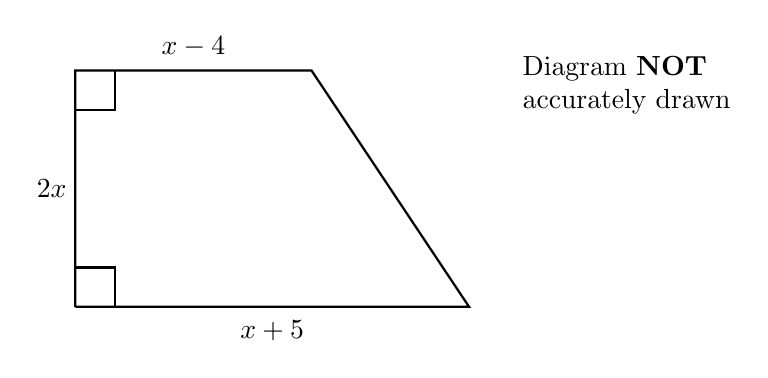
\begin{tikzpicture}
      \draw[thick] (0, 0) -- (5, 0) -- (3, 3) -- (0, 3) -- (0, 0);
      \node at (2.5, -0.3) {$x + 5$};
      \node at (-0.3, 1.5) {$2x$};
      \node at (1.5, 3.3) {$x - 4$};

      \draw[thick] (0, 0.5) -- (0.5, 0.5) -- (0.5, 0);
      \draw[thick] (0, 2.5) -- (0.5, 2.5) -- (0.5, 3);

      \node[label={[align=left]Diagram \textbf{NOT} \\ accurately drawn}] at (7, 2.2) {};
    \end{tikzpicture}
  \end{figure}
  %
  All the measurements are in centimetres.\\
  The area of the trapezium is $351 cm^2$.
  \newpage
  \begin{enumerate}
    \item Show that $2x^2 + x - 351 = 0$.\mrk{2}\strch
    \item Work out the value of $x$.\mrk{3}\strch
  \end{enumerate}
  \item Here are two triangles $\vb{T_1}$ and $\vb{T_2}$.
  %
  \begin{figure}[H]
    \centering
    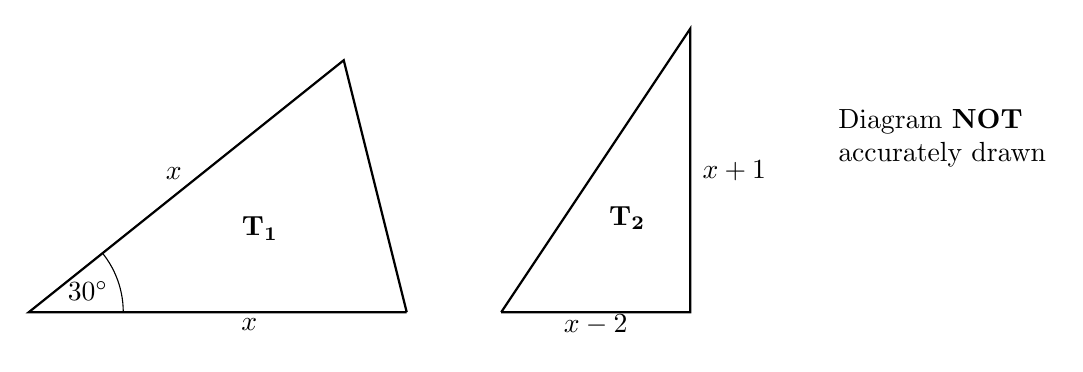
\begin{tikzpicture}[scale=0.8]
      \coordinate (A) at (-1, 0);
      \coordinate (B) at (-7, 0);
      \coordinate (C) at (-2, 4);

      \coordinate (X) at (0.5, 0);
      \coordinate (Y) at (3.5, 0);
      \coordinate (Z) at (3.5, 4.5);

      \coordinate (a1) at (-3.5, -0.2);
      \coordinate (a2) at (-4.7, 2.2);

      \coordinate (x1) at (2, -0.2);
      \coordinate (x2) at (4.2, 2.25);

      \coordinate (text) at (7.5, 2);

      \draw[thick] (A) -- (B) -- (C) -- (A);
      \draw[thick] (X) -- (Y) -- (Z) -- (X);

      \node at (-3.33, 1.33) {$\vb{T_1}$};
      \node at (2.5, 1.5) {$\vb{T_2}$};

      \begin{scope}
        \path[clip] (A) -- (B) -- (C);
        \draw (B) circle (15mm);
        \node at ($(B)+(20:10mm)$) {$\ang{30}$};
      \end{scope}

      \node at (a1) {$x$};
      \node at (a2) {$x$};

      \node at (x1) {$x - 2$};
      \node at (x2) {$x + 1$};

      \node[label={[align=left]Diagram \textbf{NOT} \\ accurately drawn}] at (text) {};
    \end{tikzpicture}
  \end{figure}
  %
  The lengths of the sides are in centimetres.\\
  The area of triangle $\vb{T_1}$ is equal to the area of triangle $\vb{T_2}$.\\
  Work out the value of $x$, giving your answer in the form $a + \sqrt{b}$ where $a$ and $b$ are integers.\strch
  \item Prove algebraically that the difference between the squares of any two consecutive integers is equal to the sum of these two integers.\strch
  \newpage
  \item \mbox{}
  \begin{figure}[H]
    \centering
    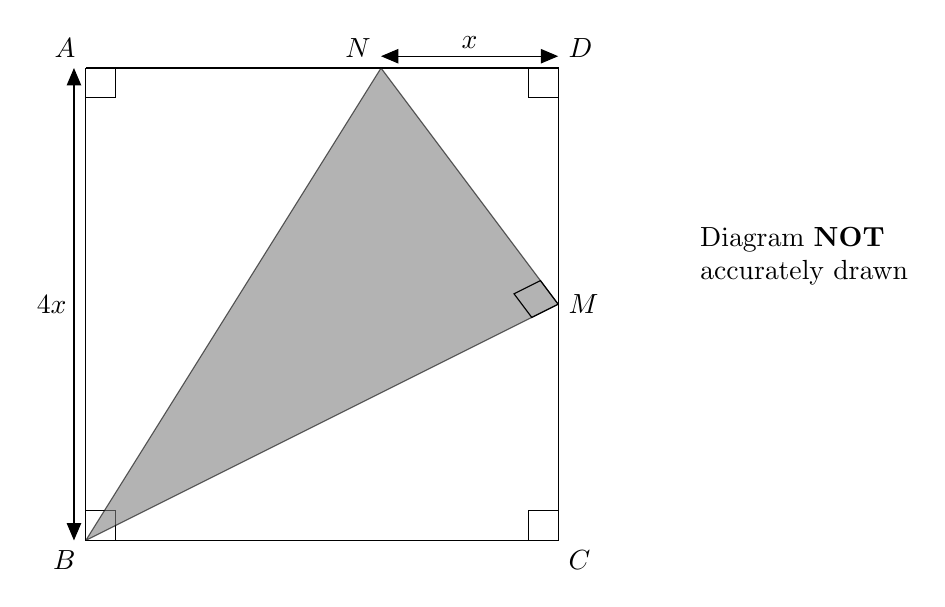
\begin{tikzpicture}[scale=1.5]
      \coordinate (B) at (0, 0);
      \coordinate (A) at (0, 4);
      \coordinate (C) at (4, 0);
      \coordinate (D) at (4, 4);

      \coordinate (M) at (4, 2);
      \coordinate (N) at (2.5, 4);

      \coordinate (varr1) at (0-0.1, 4);
      \coordinate (varr2) at (0-0.1, 0);

      \coordinate (harr1) at (4, 4+0.1);
      \coordinate (harr2) at (2.5, 4+0.1);

      \coordinate (t1) at (0, 2);
      \coordinate (t2) at (3.25, 4);

      \draw (A) -- (B) -- (C) -- (D) -- (A);

      \node at (A) [above left = 0.1mm of A] {$A$};
      \node at (B) [below left = 0.1mm of B] {$B$};
      \node at (C) [below right = 0.11mm of C] {$C$};
      \node at (D) [above right = 0.1mm of D] {$D$};

      \tkzMarkRightAngle (A,B,C);
      \tkzMarkRightAngle (B,C,D);
      \tkzMarkRightAngle (D,A,B);
      \tkzMarkRightAngle (A,D,C);

      \draw[color=black, fill=gray, opacity=0.6] (B) -- (M) -- (N) -- (B);
      \tkzMarkRightAngle (B,M,N);

      \node at (M) [right = 0.1mm of M] {$M$};
      \node at (N) [above left = 0.1mm of N] {$N$};

      \draw[>=triangle 45, <->] (varr1) -- (varr2);
      \draw[>=triangle 45, <->] (harr1) -- (harr2);

      \node at (t1) [left = 1.2mm of t1] {$4x$};
      \node at (t2) [above = 1.2mm of t2] {$x$};

      \node[label={[align=left]Diagram \textbf{NOT} \\ accurately drawn}] at (M) [right = 3cm of M] {};
    \end{tikzpicture}
  \end{figure}
  %
  $ABCD$ is a square with a side length of $4x$.\\
  $M$ is the midpoint of $DC$.\\
  $N$ is the point on $AD$ where $ND = x$.\par
  $BMN$ is a right-angled triangle.\par
  Find an expression, in terms of $x$, for the area of triangle $BMN$.\\
  Give your expression in its simplest form.\strch
  \newpage
  \item \mbox{}
  \begin{figure}[H]
    \centering
    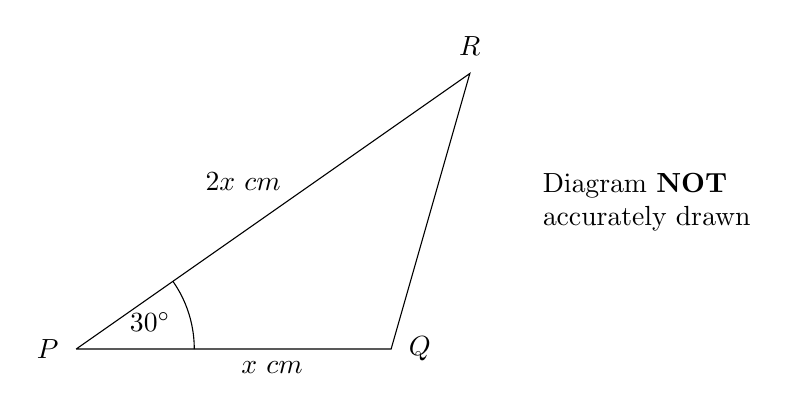
\begin{tikzpicture}
      \coordinate (P) at (0, 0);
      \coordinate (Q) at (4, 0);
      \coordinate (R) at (5, 3.5);

      \draw (P) -- (Q) -- (R) -- (P);

      \node at (P) [left = 1mm of P] {$P$};
      \node at (R) [above = 1mm of R] {$R$};
      \node at (Q) [right = 1mm of Q] {$Q$};

      \begin{scope}
        \path[clip] (R) -- (P) -- (Q);
        \draw (P) circle (15mm);
        \node at ($(P)+(20:10mm)$) {$\ang{30}$};
      \end{scope}

      \node at ($(P)+(45:3cm)$) {$2x\ cm$};
      \node at ($(P)+(-5.5:2.5cm)$) {$x\ cm$};

      \node[label={[align=left]Diagram \textbf{NOT} \\ accurately drawn}] at (R) [below right = 3cm of R] {};
    \end{tikzpicture}
  \end{figure}
  %
  $PQ = x\ cm$\\
  $PR = 2x\ cm$\\
  Angle $QPR = \ang{30}$\par
  The area of triangle $PQR = A\ cm^2$\\
  Show that $x = \sqrt{2A}$.\strch
  \item \mbox{}
  \begin{figure}[H]
    \centering
    \begin{tikzpicture}[scale=1.2]
      \coordinate (P) at (0, 0);
      \coordinate (Q) at (6, 0);
      \coordinate (R) at (0, 3);

      \draw (P) -- (Q) -- (R) -- (P);

      \tkzMarkRightAngle (R,P,Q);

      \node at ($(P)+(32:3.7cm)$) {$3x + 1$};
      \node at ($(P)+(-5.5:2.5cm)$) {$3x$};
      \node at ($(P)+(110:1.5cm)$) {$x-1$};

      \node[label={[align=left]Diagram \textbf{NOT} \\ accurately drawn}] at (Q) [above right = 3cm of Q] {};
    \end{tikzpicture}
  \end{figure}
  %
  In the diagram, all the measurements are in metres.\par
  The perimeter of the triangle is $56$ m.\\
  The area of the triangle is $A$ $\text{m}^2$.\par
  Work out the value of $A$.\strch
  \newpage
  \item \mbox{}
  \begin{figure}[H]
    \centering
    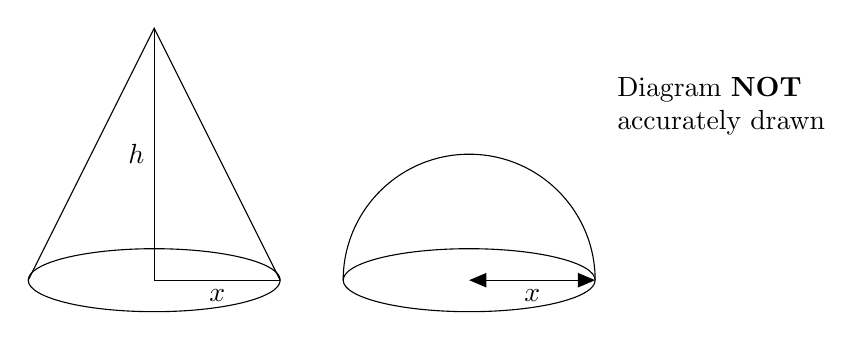
\begin{tikzpicture}[scale=0.8]
      \draw (0,0) circle (2cm and 0.5cm);
      \draw(2,0) -- (0,4) -- (-2,0);
      \draw (2,0) -- node[below] {$x$} (0,0) -- node[left] {$h$} (0,4) ;

      \draw (5,0) circle (2cm and 0.5cm);
      \draw (3,0) arc (180:0:2);

      \draw[>=triangle 45, <->] (5,0) -- node[below] {$x$} (7,0);

      \node[label={[align=left]Diagram \textbf{NOT} \\ accurately drawn}] at (9, 2) {};
    \end{tikzpicture}
  \end{figure}
  %
  The diagram shows a solid cone and a solid hemisphere.\\
  The cone has a base of radius $x$ cm and a height of $h$ cm.\\
  The hemisphere has a base of radius $x$ cm.\\
  The surface area of the cone is equal to the surface area of the hemisphere.\par
  Find an expression for $h$ in terms of $x$.\strch
  \item Umar thinks $(a + 1)^2 = a^2 + 1$ for all values of $a$.
  \begin{enumerate}
    \item Show that Umar is wrong.\mrk{2}\strch
    \item Here are two right-angled triangles.\\
    All the measurements are in centimetres
    \begin{figure}[H]
      \centering
      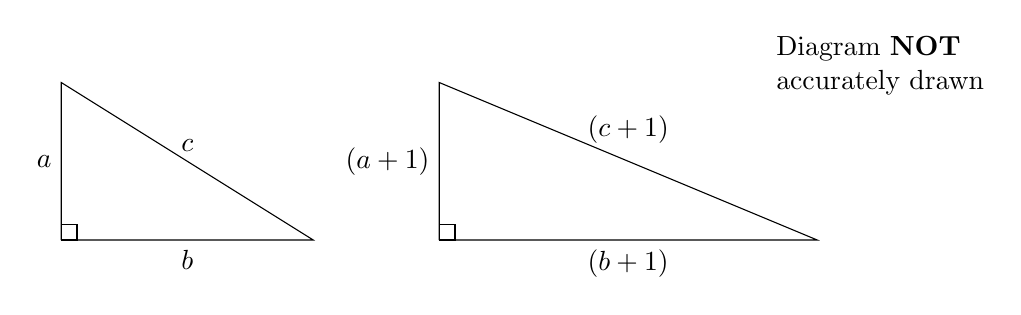
\begin{tikzpicture}[scale=0.8]
        \coordinate (A1) at (0, 0);
        \coordinate (B1) at (4, 0);
        \coordinate (C1) at (0, 2.5);

        \coordinate (A2) at (6, 0);
        \coordinate (B2) at (12, 0);
        \coordinate (C2) at (6, 2.5);

        \draw (A1) -- node[left] {$a$} (C1) -- node[above] {$c$} (B1) -- node[below] {$b$} (A1);
        \tkzMarkRightAngle (B1,A1,C1);

        \draw (A2) -- node[left] {$(a+1)$} (C2) -- node[above=1mm] {$(c+1)$} (B2) -- node[below] {$(b+1)$} (A2);
        \tkzMarkRightAngle (B2,A2,C2);

        \node[label={[align=left]Diagram \textbf{NOT} \\ accurately drawn}] at (13, 2) {};
      \end{tikzpicture}
    \end{figure}
    %
    Show that $2a + 2b + 1 = 2c$. $a,\ b$ and $c$ cannot all be integers.\mrk{3}\strch
    \newpage
    \item Explain why.\mrk{1}\strch
  \end{enumerate}
  \item The diagram below shows a large rectangle of length $(2x + 6)$ cm and width $x$ cm. A smaller rectangle of length $x$ cm and width $3$ cm is cut out and removed.
  %
  \begin{figure}[H]
    \centering
    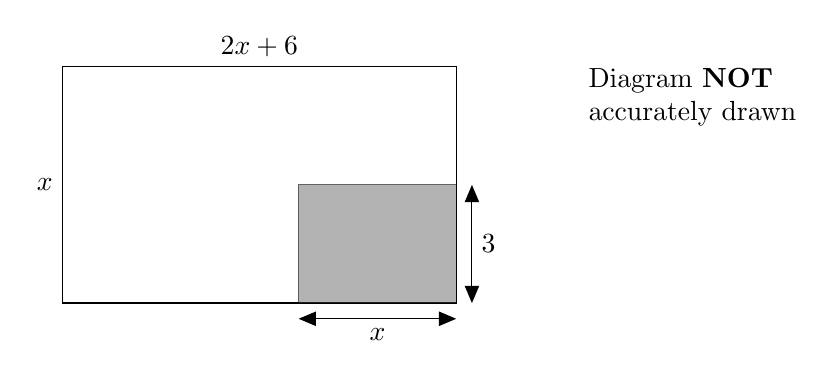
\begin{tikzpicture}
      \coordinate (A1) at (0, 0);
      \coordinate (B1) at (5, 0);
      \coordinate (C1) at (5, 3);
      \coordinate (D1) at (0, 3);

      \coordinate (A2) at (3, 0);
      \coordinate (B2) at (3, 1.5);
      \coordinate (C2) at (5, 1.5);

      \coordinate (varr1) at (3, -0.2);
      \coordinate (varr2) at (5, -0.2);

      \coordinate (harr1) at (5.2, 0);
      \coordinate (harr2) at (5.2, 1.5);

      \draw (A1) -- (B1) -- (C1) -- node[above] {$2x + 6$} (D1) -- node[left] {$x$} (A1);
      \draw[color=black, fill=gray, opacity=0.6] (A2) -- (B2) -- (C2) -- (B1) -- (A2);

      \draw[>=triangle 45, <->] (varr1) -- node[below] {$x$} (varr2);
      \draw[>=triangle 45, <->] (harr1) -- node[right] {$3$} (harr2);
    
      \node[label={[align=left]Diagram \textbf{NOT} \\ accurately drawn}] at (8, 2) {};
    \end{tikzpicture}
  \end{figure}
  %
  The area of the shape that is left is $100$ $\text{cm}^2$
  \begin{enumerate}
    \item Show that $2x^2 + 3x - 100 = 0$.\mrk{3}\strch
    \item Calculate the length of the smaller rectangle. Give your answer correct to $3$ significant figures.\mrk{4}\strch
  \end{enumerate}
  \newpage
  \item \mbox{}
  \begin{figure}[H]
    \centering
    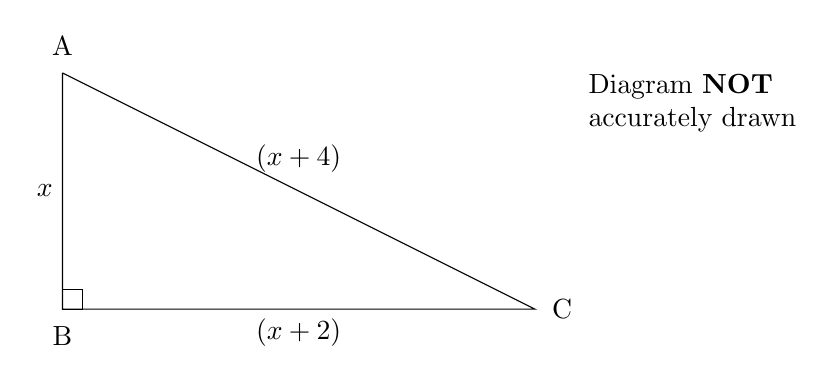
\begin{tikzpicture}
      \coordinate (B1) at (0, 0);
      \coordinate (A1) at (0, 3);
      \coordinate (C1) at (6, 0);

      \draw (A1) -- node[left] {$x$} (B1) -- node[below] {$(x+2)$} (C1) -- node[above=1.1mm] {$(x+4)$} (A1);
      \tkzMarkRightAngle (A1,B1,C1);

      \node[label=above:A, scale=0.75] (A1) at (A1) {};
      \node[label=below:B, scale=0.75] (B1) at (B1) {};
      \node[label=right:C, scale=0.75] (C1) at (C1) {};

      \node[label={[align=left]Diagram \textbf{NOT} \\ accurately drawn}] at (8, 2) {};
    \end{tikzpicture}
  \end{figure}
  %
  ABC is a right-angled triangle.\\
  All the measurements are in centimetres.\par
  $AB = x$\\
  $BC = (x + 2)$\\
  $AC = (x + 4)$
  \begin{enumerate}
    \item Show that $x^2 - 4x - 12 = 0$.\mrk{3}\strch
    \item \hfill\mrk{4}
    \begin{enumerate}
      \item Solve $x^2 - 4x - 12 = 0$\strch
      \item Hence, write down the length of $AC$.\strch
    \end{enumerate}
  \end{enumerate}
  \item Prove that the difference between the squares of two consecutive odd numbers is a multiple of $8$.\strch
  \newpage
  \item Prove that $n^2 + n + 1$ is always odd for all integers $n$.\strch
  \item Factorise $2t^2 + 5t + 2$. Hence explain why $2t^2 + 5t + 2$ can never be a prime number for any positive whole number value of $t$.\strch
\end{enumerate}
  % 
\chapter{GCSE Revision - Algebra - (Excluding Geometric problems and proofs)}
\begin{enumerate}
  \item
  \begin{enumerate}
    \item Simplify $x^7 \times x^3$\strch
    \item Simplify $(m^4)^3$\strch
    \item Simplify $\dfrac{36af^8}{12a^5f^2}$\strch\\ \vspace*{0pt}\lmrk{1}{7}
  \end{enumerate}
  \pagebreak
  \item %
  \begin{enumerate}
    \item Solve $\dfrac{4(8x - 2)}{3x} = 10$\mrk{3}\strch
    \item Write as a single fraction in its simplest form\mrk{3}
    $$
    \frac{2}{y + 3} - \frac{1}{y - 6}
    $$
    \strch
  \end{enumerate}
  %
  \item Solve the simultaneous equations
  \begin{align*}
    3x + 4y = 5\\
    2x - 3y = 9
  \end{align*}
  \hfill$x =\ $\dline\\
  \vspace*{0pt}\hfill$y =\ $\dline\\
  \vspace*{0pt}\lmrk{3}{4}
  \strch
  \item %
  \begin{align*}
    &A = 4bc\\
    &A = 100\\
    &b = 2
  \end{align*}
  \begin{enumerate}
    \item Work out the value of $c$.\mrk{2}\strch\newpage
    \item Make $k$ the subject of the formula, $m = \sqrt{\dfrac{k+1}{4}}$.\mrk{3}\strch
  \end{enumerate}
  \item Solve $\dfrac{4x - 1}{5} + \dfrac{x + 4}{2} = 3$\mrk{3}\strch\\
  \vspace*{0cm}\hfill$x =\ $\dline
  \item %
  \begin{enumerate}
    \item Simplify $a^4\times a^5$\mrk{1}\strch
    \item Simplify $\dfrac{45e^6f^8}{5ef^2}$\mrk{2}\strch
    \item Write down the value of $9^{\frac{1}{2}}$.\mrk{1}\strch
  \end{enumerate}
  \newpage
  \item Solve the simultaneous equations\mrk{6}
  \begin{align*}
    x^2 + y^2 &= 9\\
    x + y &= 2
  \end{align*}
  Give your answers correct to 2 decimal places.\strch\\
  \vspace*{0pt}\hfill$x =\ $\dline\hspace{0.2cm} $y =\ $\dline\\
  \vspace*{0pt}\hfill or $x =\ $\dline\hspace{0.2cm} $y =\ $\dline
  \item Make $p$ the subject of the formula $y = 3p^2 - 4$.\mrk{3}\strch
  \item %
  \begin{enumerate}
    \item Factorise	$6 + 9x$.\mrk{1}\strch
    \item Factorise	$y^2 - 16$.\mrk{1}\strch
    \item Factorise	$2p^2 - p - 10$.\mrk{2}\strch
  \end{enumerate}
  \newpage
  \item Solve $\dfrac{2 - y}{5} = 1$.\mrk{5}\strch\\\vspace*{0pt}\hfill $y =\ $\dline
  \item The expression $x^2 - 8x + 21$ can be written in the form $(x - a)^2 + b$ for all values of $x$.
  \begin{enumerate}
    \item Find the value of $a$ and the value of $b$.\mrk{3}\strch\\
    \vspace*{0pt}\hfill $a =\ $\dline\\
    \vspace*{0pt}\hfill $b =\ $\dline
    \suspend{enumerate}
    The equation of a curve is $y = f(x)$ where $f(x) = x^2 - 8x + 21$. The diagram shows part of a sketch of the graph of $y = f(x)$.
    \begin{figure}[H]
      \centering
      \begin{tikzpicture}
        \begin{axis}[
            xmin = -1, xmax = 10,
            ymin = -2, ymax = 30,
            xticklabels = {},
            yticklabels = {},
            axis lines = middle,
            xlabel = {$x$},
            ylabel = {$y$},
          ]
          % Plot a function
          \addplot[
            domain = -0.8:8.8,
            samples = 200,
            smooth,
            thick,
          ] {x^2 - 8*x + 21};
          \node at (7.5, 28) {$y = f(x)$};
          \node at (-0.4, -1) {$O$};
          \node at (4, 3) {$M$};
          \addplot[
            mark=x,
            mark size=6pt
          ]
          coordinates {
            (4, 5)
          };
        \end{axis}
      \end{tikzpicture}
    \end{figure}
    The minimum point of the curve is $M$.
    \resume{enumerate}
    \item Write down the coordinates of $M$.\mrk{1}\strch\\
    \vspace*{0pt}\hfill (
      \tikz\draw[thick, dashed] (0,0) -- (1.5,0);, \tikz\draw[thick, dashed] (0,0) -- (1.5,0);
    )
  \end{enumerate}
  \newpage
  \item Simplify $\dfrac{4(x + 5)}{x^2 + 2x - 15}$.\mrk{2}\strch
  \item Solve the simultaneous equations\mrk{4}
  \begin{align*}
    4x + 7y &= 1\\
    3x + 10y &= 15
  \end{align*}\strch\\
  \vspace*{0pt}\hfill$x =\ $\dline\\
  \vspace*{0pt}\hfill$y =\ $\dline
  \begin{enumerate}
    \item Solve 	$2x^2 + 9x - 7 = 0$. Give your solutions correct to 3 significant figures.\mrk{3}\strch
    \item Solve $\dfrac{2}{y^2} + \dfrac{9}{y} - 7 =0$. Give your solutions correct to 3 significant figures.\mrk{2}\strch
  \end{enumerate}
  \item Simplify $\dfrac{x + 1}{2} + \dfrac{x + 3}{3}$.\mrk{3}\strch
  \newpage
  \item %
  \begin{enumerate}
    \item %
    \begin{enumerate}
      \item Factorise $2t^2 + 5t + 2$.\strch
      \item $t$ is a positive whole number.\par
      The expression $2t^2 + 5t + 2$ can never have a value that is a prime number. Explain why.\mrk{3}\strch
    \end{enumerate}
  \end{enumerate}
  \item Make $t$ the subject of the formula\mrk{4} $$p = \frac{3-2t}{4 + t}$$\strch
  \item Solve $\dfrac{5(2x + 1)^2}{4x + 5} = 5x - 1$.\mrk{5}\strch
  \item Solve the equations\mrk{4}
  \begin{align*}
    3x + 5y &= 19\\
    4x - 2y &= -18
  \end{align*}
  \strch\\
  \vspace*{0pt}\hfill$x =\ $\dline\\
  \vspace*{0pt}\hfill$y =\ $\dline
  \item Solve the equation 	$5x^2 + 8x - 6 = 0$. Give each solution correct to 2 decimal places.\mrk{3}\strch
  \newpage
  \item %
  \begin{enumerate}
    \item On the number line below, show the inequality $-2 < y < 3$.\mrk{1}
    \begin{figure}[H]
      \centering
      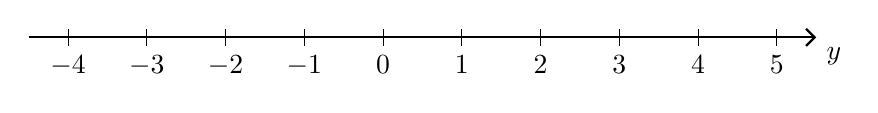
\begin{tikzpicture}
        \draw[-Straight Barb, thick] (-4.5, 0) -- (5.5, 0) node[anchor=north west] {$y$};
        \foreach \x in {-4, -3, -2, -1, 0, 1, 2, 3, 4, 5}
          \draw (\x cm, 3pt) -- (\x cm, -3pt) node[anchor=north] {$\x$};
      \end{tikzpicture}
    \end{figure}\strch
    \item Here is an inequality, in $x$, shown on a number line.\mrk{2}
    \begin{figure}[H]
      \centering
      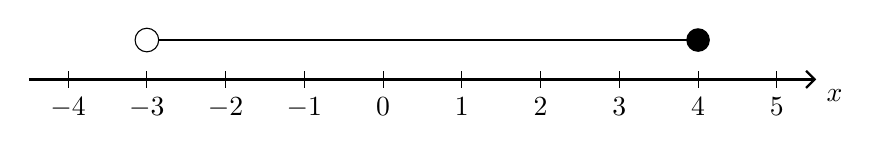
\begin{tikzpicture}
        \draw[-Straight Barb, thick] (-4.5, 0) -- (5.5, 0) node[anchor=north west] {$x$};
        \foreach \x in {-4, -3, -2, -1, 0, 1, 2, 3, 4, 5}
          \draw (\x cm, 3pt) -- (\x cm, -3pt) node[anchor=north] {$\x$};
        \draw[thick] (-3, 0.5) -- (4, 0.5);
        \filldraw[fill=white, draw=black] (-3, 0.5) circle (0.15cm);
        \fill[black] (4, 0.5) circle (0.15cm);
      \end{tikzpicture}
    \end{figure}
    Write down the inequality.\strch
    \item Solve the inequality $4t - 5 > 9$.\mrk{2}\strch
  \end{enumerate}
  \item %
  \begin{enumerate}
    \item Factorise fully $2x^2 - 4xy$.\mrk{2}\strch
    \item Factorise $p^2 - 6p + 8$.\mrk{2}\strch
    \item Simplify $\dfrac{(x+2)^2}{x+2}$.\mrk{1}\strch
    \item Simplify $2a^2b \times 3a^3b$.\mrk{2}\strch
  \end{enumerate}
  \newpage
  \item Solve $3x^2 - 4x - 2 = 0$ Give your solutions correct to 3 significant figures.\mrk{3}\strch
  \item Make $t$ the subject of the formula $2(d - t) = 4t + 7$.\mrk{3}\strch\\
  \vspace*{0pt}\hfill$t =\ $\dline
  \item %
  \begin{enumerate}
    \item Simplify fully $\dfrac{x^2 + 3x - 4}{2x^2 - 5x + 3}$.\mrk{3}\strch
    \item Write $\dfrac{4}{x + 2} + \dfrac{3}{x - 2}$ as a single fraction in its simplest form.\mrk{3}\strch
  \end{enumerate}
  \item %
  \begin{enumerate}
    \item Factorise $x^2 + px + qx + pq$.\mrk{2}\strch
    \item Factorise $m^2 - 4$.\mrk{1}\strch
    \item Write as a single fraction in its simplest form $\dfrac{2}{x - 4} - \dfrac{1}{x + 3}$.\mrk{3}\strch
  \end{enumerate}
  \newpage
  \item Find the exact solutions of $x + \dfrac{3}{x} = 7$.\mrk{3}\strch
  \item 	$-2 \leq n < 5$, $n$ is an integer.
  \begin{enumerate}
    \item Write down all the possible values of $n$.\mrk{2}\strch
    \item Solve the inequality	$4x + 1 > 11$.\mrk{2}\strch
  \end{enumerate}
  \item Simplify $(2n^3)^4$.\mrk{2}\strch
  \item %
  \begin{enumerate}
    \item Factorise $2x^2 - 9x + 4$.\mrk{2}\strch\\
    Hence, or otherwise,
    \item Solve $2x^2 - 9x + 4 = (2x - 1)^2$\mrk{4}\strch
  \end{enumerate}
  \newpage
  \item $y = p - 2qx^2$\par
  $p = -10,\quad q = 3,\quad	x = -5$    
  \begin{enumerate}
    \item Work out the value of $y$.\mrk{2}\strch
    \item Rearrange $y = p - 2qx^2$ to make $x$ the subject of the formula.\mrk{3}\strch
  \end{enumerate}
  \item The diagram shows the graph of $y = x^2 - 5x - 3$
  \begin{figure}[H]
    \centering
    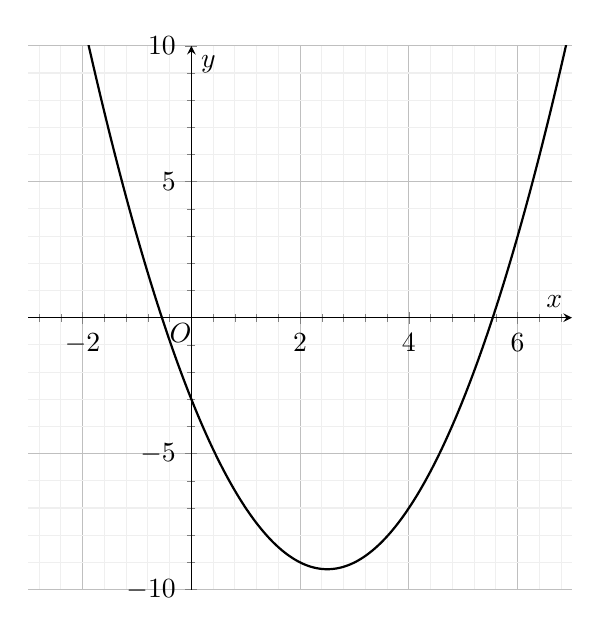
\begin{tikzpicture}
      \begin{axis}[
          xmin = -3, xmax = 7,
          ymin = -10, ymax = 10,
          grid = both,
          minor tick num = 4,
          major grid style = {lightgray},
          minor grid style = {lightgray!25},
          axis lines = center,
          width = 0.7\textwidth,
          height = 0.7\textwidth,
          xlabel = {$x$},
          ylabel = {$y$},
        ]
        % Plot a function
        \addplot[
          domain = -2:7,
          samples = 500,
          smooth,
          thick,
        ] {x^2 - 5*x - 3};
        \node at (-0.2, -0.55) {$O$};
      \end{axis}
    \end{tikzpicture}
  \end{figure}
  \newpage
  \begin{enumerate}
    \item Use the graph to find estimates for the solutions of.\mrk{3}
    \begin{enumerate}
      \item $x^2 - 5x - 3 = 0$.\strch
      \item $x^2 - 5x - 3 = 6$.\strch
    \end{enumerate}
    \item Use the graph to find estimates for the solutions of the simultaneous equations\mrk{3}
    \begin{align*}
      y &= x2 - 5x - 3\\
      y &= x - 4
    \end{align*}\strch
  \end{enumerate}
  \item The table shows six expressions. $n$ is a positive integer.\par
  \begin{table}[H]
    \centering
    \resizebox{0.85\textwidth}{!}{%
    \begin{tabular}{|c|c|c|c|c|c|} 
      \hline
      $2n - 3$ & $3n - 2$ & $3(n + 4)$ & $4n + 1$ & $4(3n + 1)$ & $2n + 1$ \\ 
      \hline
    \end{tabular}}
  \end{table}
  \begin{enumerate}
    \item From the table, write the expression whose value is\mrk{2}
    \begin{enumerate}
      \item always even.
      \item always a multiple of 3.
    \end{enumerate}
    \item From the table, write the expression which is a factor of $4n^2 - 1$.\mrk{1}\strch
  \end{enumerate}
  \item Solve the equation $\dfrac{x}{2} - \dfrac{2}{x + 1} = 1$.\mrk{4}\strch
  \newpage
  \item Make $k$ the subject of the formula $t = \dfrac{k}{k - 2}$.\mrk{4}\strch
  \item %
  \begin{enumerate}
    \item Simplify completely $\dfrac{12xy^3}{3x^2y^3}$.\mrk{2}\strch
  \end{enumerate}
  \item %
  \begin{enumerate}
    \item Expand and simplify $(2x + 4y)(4x - 5y)$.\mrk{2}\strch
    \item Simplify fully $\dfrac{(x + 10)^5}{(x + 10)^4}$.\mrk{1}\strch
    \item Simplify fully $\dfrac{x^2 - 25}{x^2 + 7x + 10}$\mrk{3}\strch
    \item For all values of $x,\ x^2 + 6x - 2 = (x + p)^2 + q$. Find the value of $p$ and the value of $q$.\mrk{3}\strch\\
    \vspace*{0pt}\hfill $p=\ $
      \tikz\draw[thick, dashed] (0,0) -- (1.5,0);, $q=\ $ \tikz\draw[thick, dashed] (0,0) -- (1.5,0);
  \end{enumerate}
  \newpage
  \item Make $v$ the subject of the formula $t = \dfrac{v}{5} + 2$.\mrk{2}\\[2cm]
  \vspace*{0pt}\hfill $v=\ $\dline
\end{enumerate}
  % 
\chapter{GCSE Revision - Angles (and Bearings)}

\begin{enumerate}
  \item \mrk{4}
  \begin{figure}[H]
    \centering
    \begin{tikzpicture}[scale=1.3]
      \tkzDefPoints{-4/0/P,1/0/Q,0/2/T,3/0/R,5/1.8/L}
      \tkzDrawPolygon(P,Q,T)
      \tkzDrawSegments(Q,R)
      \tkzMarkAngle[size=0.6, mark=none](R,Q,T)
      \tkzMarkAngle[size=1, mark=none](Q,P,T)
      \tkzMarkSegments[mark=|](P,Q P,T)

      \tkzLabelAngle[pos=0.3](R,Q,T){\small $\ang{110}$}
      \tkzLabelAngle[pos=0.7](Q,P,T){\small $y^\circ$}
      \tkzLabelPoints[below](P,Q,R)
      \tkzLabelPoint[above](T){T}
      \tkzLabelPoint[above](L){Diagram \textbf{NOT}}
      \tkzLabelPoint[below](L){accurately drawn}
    \end{tikzpicture}
  \end{figure}
  $PQR$ is a straight line. $PT = PQ$.
  \begin{enumerate}
    \item Work out the value of $y$.\strch\\\vspace*{0cm}\hfill\dline
    \item Give reasons for your answer.\\
    \hdashrule{0.85\textwidth}{1pt}{1ex}\\
    \hdashrule{0.85\textwidth}{1pt}{1ex}\strch
  \end{enumerate}

  \newpage
  \item \mrk{4}
  \begin{figure}[H]
    \centering
    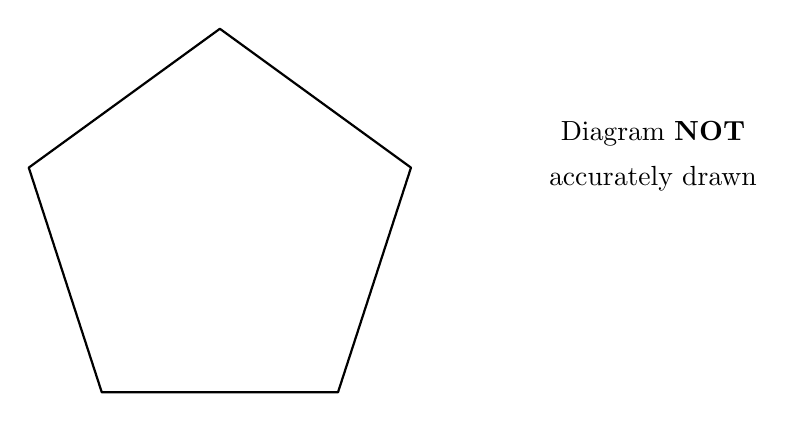
\begin{tikzpicture}
      \tkzDefPoints{0/0/A, 3/0/B, 7/3/L}
      \tkzDefRegPolygon[side,sides=5,name=P](A,B)
      \tkzDrawPolygon[thick](P1,P...,P5)
      \tkzLabelPoint[above](L){Diagram \textbf{NOT}}
      \tkzLabelPoint[below](L){accurately drawn}
    \end{tikzpicture}
  \end{figure}
  Work out the size of an exterior angle of a regular pentagon.\strch\\\vspace*{0cm}\hfill\dline
  \item \mrk{3}
  \begin{figure}[H]
    \centering
    \begin{tikzpicture}
      \tkzDefPoints{0/0/C, 2/0/M, 6/0/D, 0/3/A, 6/3/B, 4/5/L, 9/5/P}
      \tkzInterLL(A,B)(M,L)
      \tkzGetPoint{N}
      \tkzDrawSegments[->, >=latex, thick](A,B C,D)
      \tkzDrawSegments[thick](M,L)
      \tkzMarkAngle[size=0.5, mark=none](L,N,A)
      \tkzMarkAngle[size=1, mark=none](D,M,L)

      \tkzLabelAngle[pos=0.3](L,N,A){\small $y$}
      \tkzLabelAngle[pos=0.7](D,M,L){\small $\ang{60}$}

      \tkzLabelPoint[left](A){$A$}
      \tkzLabelPoint[left](C){$C$}
      \tkzLabelPoint[right](B){$B$}
      \tkzLabelPoint[right](D){$D$}
      \tkzLabelPoint[below right](M){$M$}
      \tkzLabelPoint[below right](N){$N$}
      \tkzLabelPoint[above right](L){$L$}

      \tkzLabelPoint[above](P){Diagram \textbf{NOT}}
      \tkzLabelPoint[below](P){accurately drawn}
    \end{tikzpicture}
  \end{figure}
  $ANB$ is parallel to $CMD$. $LNM$ is a straight line. Angle $LMD = \ang{68}$.
  \begin{enumerate}
    \item Work out the size of the angle marked $y$.\strch\\\vspace*{0cm}\hfill\dline$^\circ$
    \item Give reasons for your answer.\\
    \hdashrule{0.85\textwidth}{1pt}{1ex}\\
    \hdashrule{0.85\textwidth}{1pt}{1ex}\strch
  \end{enumerate}

  \newpage
  \item \mrk{2}
  \begin{figure}[H]
    \centering
    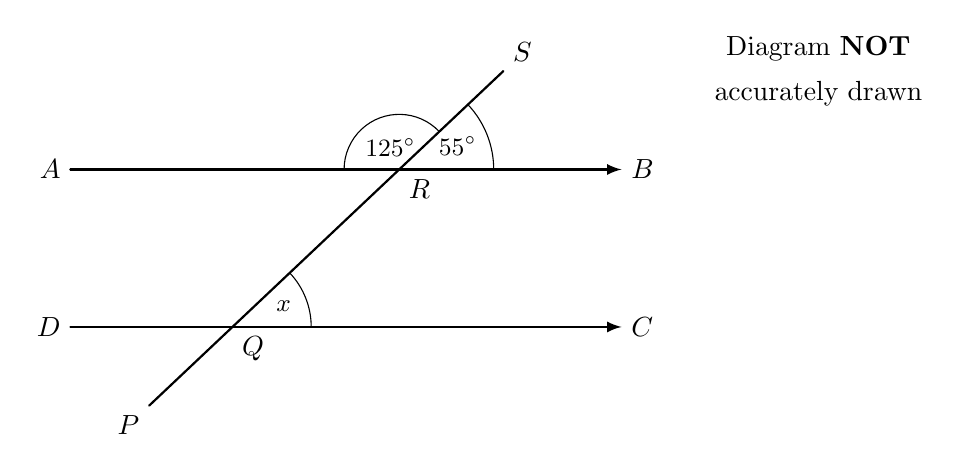
\begin{tikzpicture}
      \tkzDefPoints{0/0/D, 1/-1/P, 7/0/C, 0/2/A, 7/2/B, 5.5/3.25/S, 9.5/3.25/L}
      \tkzInterLL(A,B)(P,S)
      \tkzGetPoint{R}
      \tkzInterLL(D,C)(P,S)
      \tkzGetPoint{Q}
      \tkzDrawSegments[->, >=latex, thick](A,B D,C)
      \tkzDrawSegments[thick](P,S)
      \tkzMarkAngle[size=0.7, mark=none](S,R,A)
      \tkzMarkAngle[size=1.2, mark=none](B,R,S)
      \tkzMarkAngle[size=1, mark=none](C,Q,R)

      \tkzLabelAngle[pos=0.3](S,R,A){\small $\ang{125}$}
      \tkzLabelAngle[pos=0.8](B,R,S){\small $\ang{55}$}
      \tkzLabelAngle[pos=0.7](C,Q,R){\small $x$}

      \tkzLabelPoint[left](A){$A$}
      \tkzLabelPoint[right](C){$C$}
      \tkzLabelPoint[right](B){$B$}
      \tkzLabelPoint[left](D){$D$}
      \tkzLabelPoint[below left](P){$P$}
      \tkzLabelPoint[below right](Q){$Q$}
      \tkzLabelPoint[below right](R){$R$}
      \tkzLabelPoint[above right](S){$S$}

      \tkzLabelPoint[above](L){Diagram \textbf{NOT}}
      \tkzLabelPoint[below](L){accurately drawn}
    \end{tikzpicture}
  \end{figure}
  $ARB$ is parallel to $DQC$. $PQRS$ is a straight line. Angle $SRB = \ang{55}$.
  \begin{enumerate}
    \item Find the size of the angle marked $x$.\strch\\\vspace*{0cm}\hfill\dline$^\circ$
    \item Give a reason for your answer.\\
    \hdashrule{0.85\textwidth}{1pt}{1ex}\strch
  \end{enumerate}
  \item \mrk{3}
  \begin{figure}[H]
    \centering
    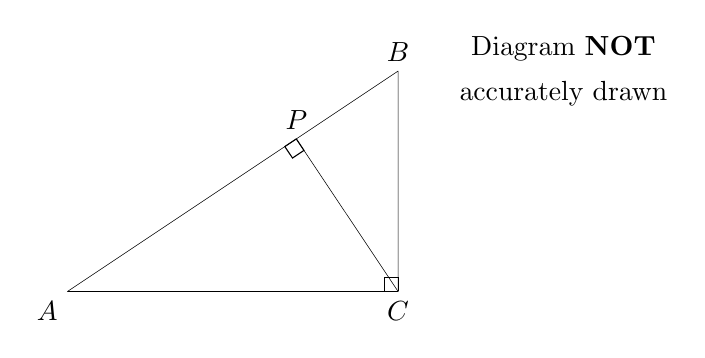
\begin{tikzpicture}[scale=0.7]
      \tkzDefPoints{0/0/A, 6/0/C, 6/4/B, 9/4/L}
      \tkzDrawPolygon(A,B,C)
      \tkzDefLine[perpendicular=through C](A,B)
      \tkzGetPoint{F}
      \tkzInterLL(A,B)(F,C)
      \tkzGetPoint{P}
      \tkzDrawSegment(C,P)

      \tkzMarkRightAngle(A,P,C)
      \tkzMarkRightAngle(A,C,B)

      \tkzLabelPoint[below left](A){$A$}
      \tkzLabelPoint[below](C){$C$}
      \tkzLabelPoint[above](B){$B$}
      \tkzLabelPoint[above](P){$P$}

      \tkzLabelPoint[above](L){Diagram \textbf{NOT}}
      \tkzLabelPoint[below](L){accurately drawn}
    \end{tikzpicture}
  \end{figure}
  In the diagram, $ABC$ is a triangle, angle $ACB = \ang{90}$, $P$ lies on the line $AB$, $CP$ is perpendicular to $AB$.\\
  Prove that the angles of triangle $APC$ are the same as the angles of triangle $CPB$.\strch

  \newpage
  \item \mrk{4}
  \begin{figure}[H]
    \centering
    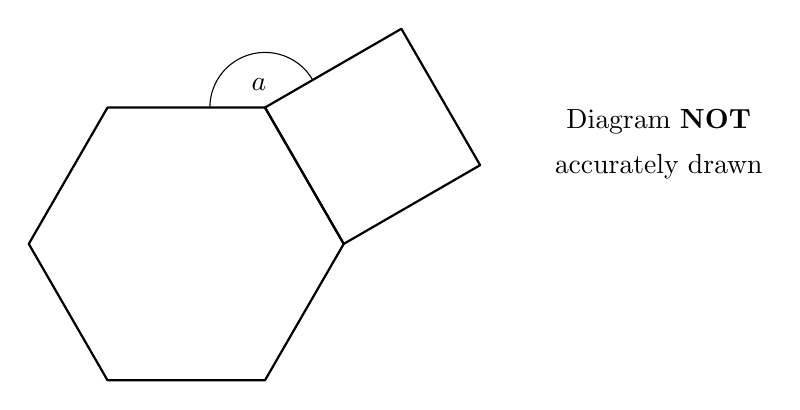
\begin{tikzpicture}
      \tkzDefPoints{0/0/A, 2/0/B, 7/3/L}
      \tkzDefRegPolygon[side,sides=6,name=P](A,B)
      \tkzDrawPolygon[thick](P1,P...,P6)

      \tkzDefSquare(P4,P3)
      \tkzGetPoints{E}{F}
      \tkzDrawPolygon[thick](P3,P4,F,E)

      \tkzMarkAngle[size=0.7, mark=none](F,P4,P5)
      \tkzLabelAngle[pos=0.3](F,P4,P5){$a$}

      \tkzLabelPoint[above](L){Diagram \textbf{NOT}}
      \tkzLabelPoint[below](L){accurately drawn}
    \end{tikzpicture}
  \end{figure}
  The diagram shows a regular hexagon and a square. Calculate the size of the angle $a$.\strch\\
  \vspace*{0cm}\hfill\dline$^\circ$
  \item \mrk{3}
  \begin{figure}[H]
    \centering
    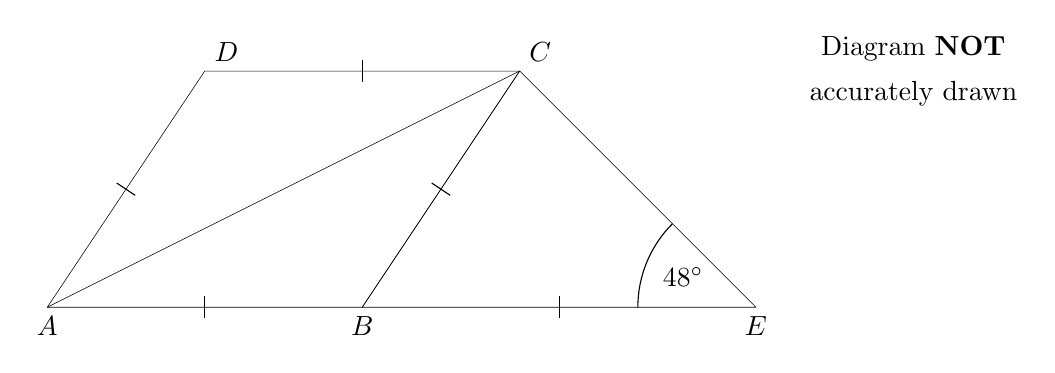
\begin{tikzpicture}
      \tkzDefPoints{0/0/A,4/0/B,6/3/C,9/0/E, 11/3/L}
      \tkzDefParallelogram(A,B,C)
      \tkzGetPoint{D}
      \tkzDrawPolygon(A,B,C,D)
      \tkzDrawPolygon(B,C,E)
      \tkzDrawSegment(A,C)

      \tkzMarkAngle[size=1.5, mark=none](C,E,B)
      \tkzLabelAngle[pos=1](C,E,B){$\ang{48}$}

      \tkzMarkSegments[mark=|](A,D A,B B,C D,C B,E)

      \tkzLabelPoints(A,B,E)
      \tkzLabelPoints[above right](C,D)

      \tkzLabelPoint[above](L){Diagram \textbf{NOT}}
      \tkzLabelPoint[below](L){accurately drawn}
    \end{tikzpicture}
  \end{figure}
  $ABCD$ is a rhombus. $BCE$ is an isosceles triangle. $ABE$ is a straight line.\\
  Work out the size of angle $DCA$.\strch\\\vspace*{0cm}\hfill\dline$^\circ$

  \newpage
  \item \mrk{7}
  \begin{figure}[H]
    \centering
    \begin{tikzpicture}
      \tkzDefPoints{0/0/A, 6/0/B, 9/0/C, 2/3/P, 11/3/L}
      \tkzDrawSegments(A,B B,C)
      \tkzDrawPolygon(A,B,P)

      \tkzMarkAngle[size=1.2, mark=none](A,P,B)
      \tkzMarkAngle[size=1.8, mark=none](B,A,P)
      \tkzMarkAngle[size=0.55, mark=none](C,B,P)

      \tkzLabelAngle[pos=0.8](A,P,B){\small $x+50$}
      \tkzLabelAngle[pos=1.2](B,A,P){\small $2x-10$}
      \tkzLabelAngle[pos=0.3](C,B,P){\small $y$}

      \tkzLabelPoints[below](A,B,C)
      \tkzLabelPoint[above](P){$P$}

      \tkzLabelPoint[above](L){Diagram \textbf{NOT}}
      \tkzLabelPoint[below](L){accurately drawn}
    \end{tikzpicture}
  \end{figure}
  All angles are measured in degrees. $ABC$ is a straight line.\\
  Angle $APB = x + 50$, Angle $PAB = x - 10$, Angle $PBC = y$.
  \begin{enumerate}
    \item Show that y = 3x + 40. Give reasons for each stage of your working.\mrk{3}\strch
    \item Given that $y = 145$\mrk{4}
    \begin{enumerate}
      \item work out the value of $x$.\strch\\\vspace*{0cm}\hfill$x=$\dline
      \item work out the size of the largest angle in triangle $ABP$.\strch\\\vspace*{0cm}\hfill\dline$^\circ$
    \end{enumerate}
  \end{enumerate}

  \newpage
  \item \mrk{3}
  \begin{figure}[H]
    \centering
    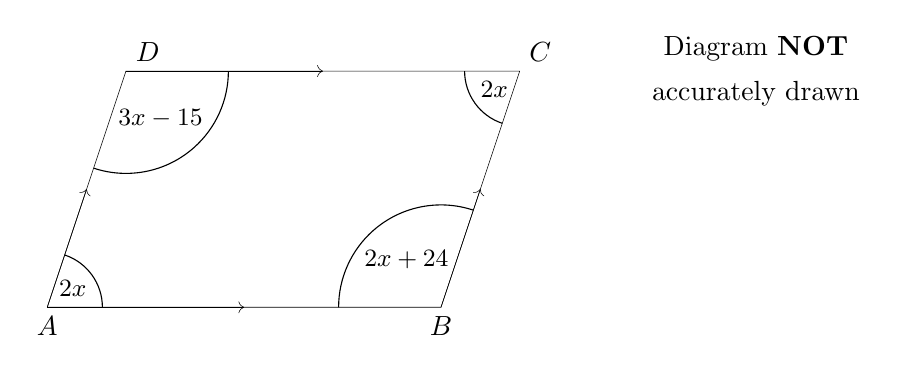
\begin{tikzpicture}
      \tkzDefPoints{0/0/A,5/0/B,6/3/C, 9/3/L}
      \tkzDefParallelogram(A,B,C)
      \tkzGetPoint{D}

      \tkzDefMidPoint(A,B)
      \tkzGetPoint{E}
      \tkzDefMidPoint(B,C)
      \tkzGetPoint{F}
      \tkzDefMidPoint(D,C)
      \tkzGetPoint{G}
      \tkzDefMidPoint(A,D)
      \tkzGetPoint{H}

      \tkzDrawSegments[->](A,E B,F D,G A,H)

      \tkzMarkAngles[size=0.7, mark=none](B,A,D D,C,B)
      \tkzMarkAngles[size=1.3, mark=none](A,D,C C,B,A)

      \tkzLabelAngle[pos=0.4](B,A,D){\small $2x$}
      \tkzLabelAngle[pos=0.4](D,C,B){\small $2x$}

      \tkzLabelAngle[pos=0.75](A,D,C){\small $3x-15$}
      \tkzLabelAngle[pos=0.75](C,B,A){\small $2x+24$}

      \tkzDrawPolygon(A,B,C,D)
      \tkzLabelPoints(A,B)
      \tkzLabelPoints[above right](C,D)

      \tkzLabelPoint[above](L){Diagram \textbf{NOT}}
      \tkzLabelPoint[below](L){accurately drawn}
    \end{tikzpicture}
  \end{figure}
  The diagram shows a parallelogram.\\
  The sizes of the angles, in degrees, are as pictured. Work out the value of $x$.\strch\\
  \vspace*{0cm}\hfill$x=$\dline
  \item \mrk{4}
  \begin{figure}[H]
    \centering
    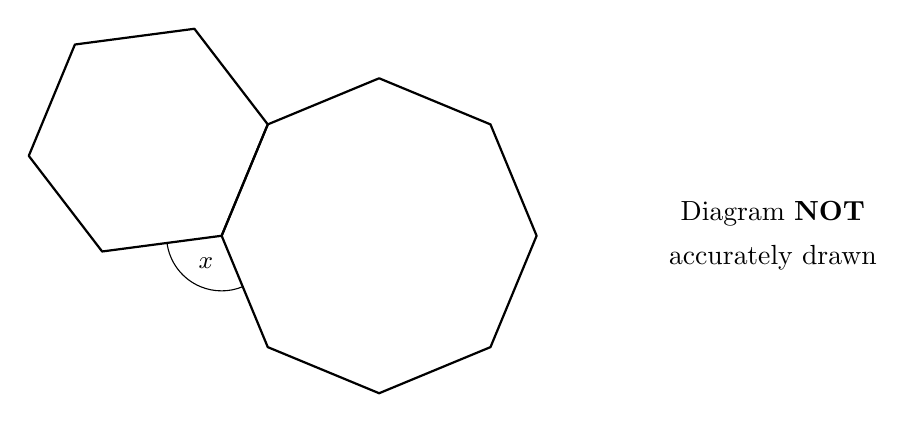
\begin{tikzpicture}
      \tkzDefPoints{0/0/A, 2/0/B, 5/0/L}
      \tkzDefRegPolygon[center,sides=8,name=P](A,B)
      \tkzDrawPolygon[thick](P1,P...,P8)

      \tkzDefRegPolygon[side,sides=6,name=Q](P5,P4)
      \tkzDrawPolygon[thick](Q1,Q...,Q6)

      \tkzMarkAngles[size=0.7, mark=none](Q6,P5,P6)
      \tkzLabelAngle[pos=0.4](Q6,P5,P6){\small $x$}

      \tkzLabelPoint[above](L){Diagram \textbf{NOT}}
      \tkzLabelPoint[below](L){accurately drawn}
    \end{tikzpicture}
  \end{figure}
  The diagram shows a regular hexagon and a regular octagon.\par
  Calculate the size of the angle marked $x$.\\
  You must show all your working.\strch\\\vspace*{0cm}\hfill\dline$^\circ$
  
  \newpage
  \item The diagram shows the position of a lighthouse $L$ and a harbour $H$.\mrk{4}
  \begin{figure}[H]
    \centering
    \begin{tikzpicture}
      \tkzDefPoints{2/2/L, 7/0/H, 2/5/N1, 7/3/N2, 10/3/P}
      \tkzDrawSegment(L,H)
      \tkzDrawSegments[->, -Triangle](L,N1 H,N2)
      \tkzDrawPoints[shape=cross out,size=4, thick](H,L)

      \tkzLabelPoints[below](L,H)
      \tkzLabelPoint[above](N1){$\vb{N}$}
      \tkzLabelPoint[above](N2){$\vb{N}$}

      \tkzLabelPoint[above](P){Diagram \textbf{NOT}}
      \tkzLabelPoint[below](P){accurately drawn}
    \end{tikzpicture}
  \end{figure}
  The scale of the diagram is $1$ cm represents $5$ km
  \begin{enumerate}
    \item Work out the real distance between $L$ and $H$.\strch\\\vspace*{0cm}\hfill\dline km
    \item Measure the bearing of $H$ from $L$.\strch\\\vspace*{0cm}\hfill\dline$^\circ$
    \suspend{enumerate}
    A boat $B$ is $20$ km from $H$ on a bearing of $\ang{040}$
    \resume{enumerate}
    \item On the diagram, mark the position of boat $B$ with a cross ($\times$). Label it $B$.\strch
  \end{enumerate}
  \item \mrk{3}
  \begin{figure}[H]
    \centering
    \begin{tikzpicture}
      \tkzDefPoints{0/3/A, 7/3/C, 0/0/D, 7/0/F, 2/3/B, 6.5/-1.5/G, 10/3/L}
      \begin{scope}[decoration={
        markings,
        mark=at position 0.2 with {\arrow{>}}}
        ]
        \tkzDrawSegments[postaction={decorate}](A,C D,F)
      \end{scope}
      \tkzDrawSegment(B,G)

      \tkzInterLL(D,F)(B,G)
      \tkzGetPoint{E}

      \tkzMarkAngles[size=0.5, mark=none](A,B,G)
      \tkzLabelAngle[pos=0.3](A,B,G){\small $x$}

      \tkzMarkAngles[size=1, mark=none](G,E,F)
      \tkzLabelAngle[pos=0.7](G,E,F){\small $\ang{47}$}

      \tkzLabelPoints[left](A, D)
      \tkzLabelPoints[right](C, F)
      \tkzLabelPoints[above](B)
      \tkzLabelPoints[below](G)
      \tkzLabelPoints[below left](E)

      \tkzLabelPoint[above](L){Diagram \textbf{NOT}}
      \tkzLabelPoint[below](L){accurately drawn}
    \end{tikzpicture}
  \end{figure}
  $ABC$ and $DEF$ are parallel lines. $BEG$ is a straight line. Angle $GEF = \ang{47}$.\\
  Work out the size of the angle marked $x$.\\
  Give reasons for your answer.\strch\\\vspace*{0cm}\hfill\dline$^\circ$
  
  \newpage
  \item \mrk{3}
  \begin{figure}[H]
    \centering
    \begin{tikzpicture}[scale=0.7]
      \tkzDefPoints{-1/1/A, 3/4/B, 7/1/C, 1.5/2/D, 9/2/E, 2/5/F, 6/0/G, 15/4/L}
      \begin{scope}[decoration={
        markings,
        mark=at position 0.9 with {\arrow[thick]{Stealth}}}
        ]
        \tkzDrawLine[postaction={decorate}, add=0.4 and 0.3](A,B)
        \tkzDefLine[parallel=through C](A,B)
        \tkzGetPoint{c'}
        \tkzDrawLine[postaction={decorate}, add=0.4 and 0.3](C,c')
      \end{scope}
      \tkzDrawLines[add=0.4 and 0.2](D,E)
      \tkzDrawLines[add=0 and 0.2](F,G)

      \tkzInterLL(D,E)(C,c')
      \tkzGetPoint{m1}
      \tkzMarkAngles[size=1, mark=none](C,m1,E)
      \tkzLabelAngle[pos=0.6](C,m1,E){$\ang{150}$}

      \tkzInterLL(F,G)(C,c')
      \tkzGetPoint{m2}
      \tkzMarkAngles[size=1.2, mark=none](G,m2,C)
      \tkzLabelAngle[pos=0.7](G,m2,C){$\ang{85}$}

      \tkzInterLL(A,B)(F,G)
      \tkzGetPoint{m3}
      \tkzMarkAngles[size=1.2, mark=none](A,m3,G)
      \tkzLabelAngle[pos=0.7](A,m3,G){\Large $y^\circ$}

      \tkzInterLL(A,B)(D,E)
      \tkzGetPoint{m4}
      \tkzMarkAngles[size=1, mark=none](A,m4,D)
      \tkzLabelAngle[pos=0.6](A,m4,D){\Large $x^\circ$}

      \tkzLabelPoint[above](L){Diagram \textbf{NOT}}
      \tkzLabelPoint[below](L){accurately drawn}
    \end{tikzpicture}
  \end{figure}
  \begin{enumerate}
    \item Find the value of $x$.\mrk{1}\strch\\\vspace*{0cm}\hfill\dline
    \item Find the value of $y$. Give reasons for your answer.\mrk{2}\strch\\\vspace*{0cm}\hfill\dline
  \end{enumerate}
  \item The bearing of a ship from a lighthouse is $0\ang{050}$. Work out the bearing of the lighthouse from the ship.\mrk{2}\strch\\\vspace*{0cm}\hfill\dline$^\circ$
  
  \newpage
  \item The diagram shows part of a pattern made from tiles.\mrk{4}
  \begin{figure}[H]
    \centering
    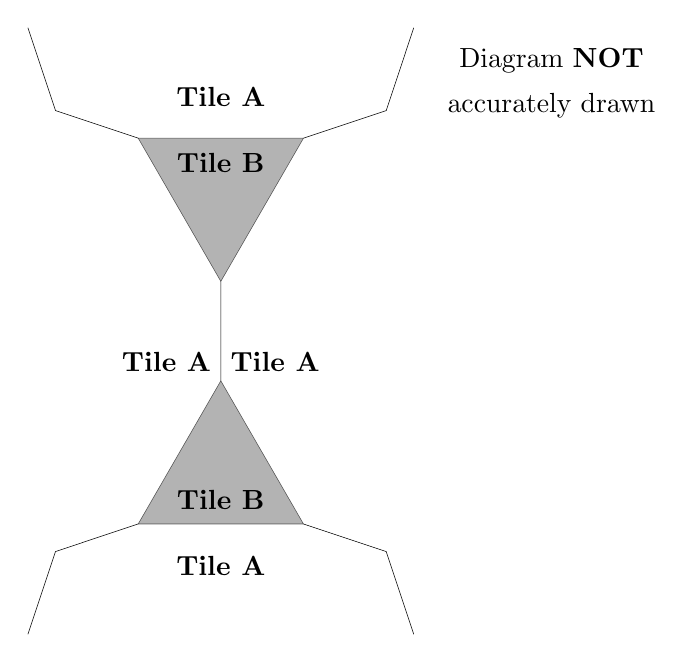
\begin{tikzpicture}[scale=0.7]
      % \tkzInit[xmax=7,ymax=10]
      % \tkzGrid[sub,orange]

      \tkzDefPoints{2/7/A,5/7/B, 0.5/7.5/D, 6.5/7.5/E}

      \tkzDefTriangle[equilateral](B,A)
      \tkzGetPoint{C}
      \tkzDrawPolygon[fill=gray, opacity=0.6](A,B,C)

      \tkzDefShiftPoint[A](0,-7){A'}
      \tkzDefShiftPoint[B](0,-7){B'}

      \tkzDefTriangle[equilateral](A',B')
      \tkzGetPoint{C'}
      \tkzDrawPolygon[fill=gray, opacity=0.6](A',B',C')

      \tkzDefShiftPoint[D](0,-8){D'}
      \tkzDefShiftPoint[E](0,-8){E'}

      \tkzDefShiftPoint[D](-0.5,1.5){F}
      \tkzDefShiftPoint[E](0.5,1.5){G}

      \tkzDefShiftPoint[D'](-0.5,-1.5){F'}
      \tkzDefShiftPoint[E'](0.5,-1.5){G'}

      \tkzDefShiftPoint[C](0,1.8){T1}
      \tkzLabelPoint[above](T1){\textbf{Tile B}}

      \tkzDefShiftPoint[C'](0,-1.8){T2}
      \tkzLabelPoint[below](T2){\textbf{Tile B}}

      \tkzDefShiftPoint[C](0,3){t1}
      \tkzLabelPoint[above](t1){\textbf{Tile A}}

      \tkzDefShiftPoint[C'](0,-3){t2}
      \tkzLabelPoint[below](t2){\textbf{Tile A}}

      \tkzLabelPoint[above left](C'){\textbf{Tile A}}
      \tkzLabelPoint[above right](C'){\textbf{Tile A}}

      \tkzDefShiftPoint[G](2.5,-1){L}

      \tkzDrawSegments(A,D B,E A',D' B',E' D,F E,G D',F' E',G' C,C')

      \tkzLabelPoint[above](L){Diagram \textbf{NOT}}
      \tkzLabelPoint[below](L){accurately drawn}
    \end{tikzpicture}
  \end{figure}
  The pattern is made from two types of tiles, tile A and tile B.\\
  Both tile A and tile B are regular polygons. Work out the number of sides tile A has.\strch\\\vspace*{0cm}\hfill\dline
  \item \mrk{4}
  \begin{figure}[H]
    \centering
    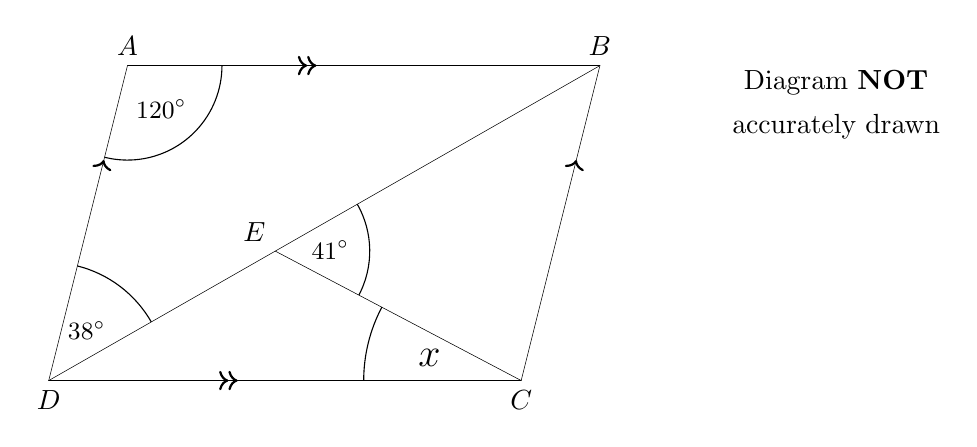
\begin{tikzpicture}
      \tkzDefPoints{0/0/D,6/0/C,7/4/B,2.2/2/F,10/3.5/L}
      \tkzDefParallelogram(D,C,B)
      \tkzGetPoint{A}

      \begin{scope}[decoration={
        markings,
        mark=at position 0.4 with {\arrow[thick]{>>}}}
        ]
        \tkzDrawSegment[postaction={decorate}](A,B)
        \tkzDrawSegment[postaction={decorate}](D,C)
      \end{scope}

      \begin{scope}[decoration={
        markings,
        mark=at position 0.7 with {\arrow[thick]{>}}}
        ]
        \tkzDrawSegment[postaction={decorate}](D,A)
        \tkzDrawSegment[postaction={decorate}](C,B)
      \end{scope}

      \tkzInterLL(D,B)(F,C)
      \tkzGetPoint{E}

      \tkzDrawSegment(C,E)
      \tkzDrawSegment(D,B)

      \tkzMarkAngles[size=1.2, mark=none](D,A,B)
      \tkzLabelAngle[pos=0.7](D,A,B){\small $\ang{120}$}

      \tkzMarkAngles[size=1.5, mark=none](B,D,A)
      \tkzLabelAngle[pos=0.8](B,D,A){\small $\ang{38}$}

      \tkzMarkAngles[size=1.2, mark=none](C,E,B)
      \tkzLabelAngle[pos=0.7](C,E,B){\small $\ang{41}$}

      \tkzMarkAngles[size=2, mark=none](E,C,D)
      \tkzLabelAngle[pos=1.2](E,C,D){\Large $x$}

      \tkzLabelPoints[above](A,B)
      \tkzLabelPoints[below](C,D)
      \tkzLabelPoints[above left](E)

      \tkzLabelPoint[above](L){Diagram \textbf{NOT}}
      \tkzLabelPoint[below](L){accurately drawn}
      \end{tikzpicture}
  \end{figure}
  $ABCD$ is a parallelogram. Angle $ADB = \ang{38}$. Angle $BEC = \ang{41}$.
  Angle $DAB = \ang{120}$. Calculate the size of angle $x$. You must give reasons for your answer.\strch

  \newpage
  \item Here is a map. The position of a ship, $S$, is marked on the map.\mrk{3}
  \begin{figure}[H]
    \centering
    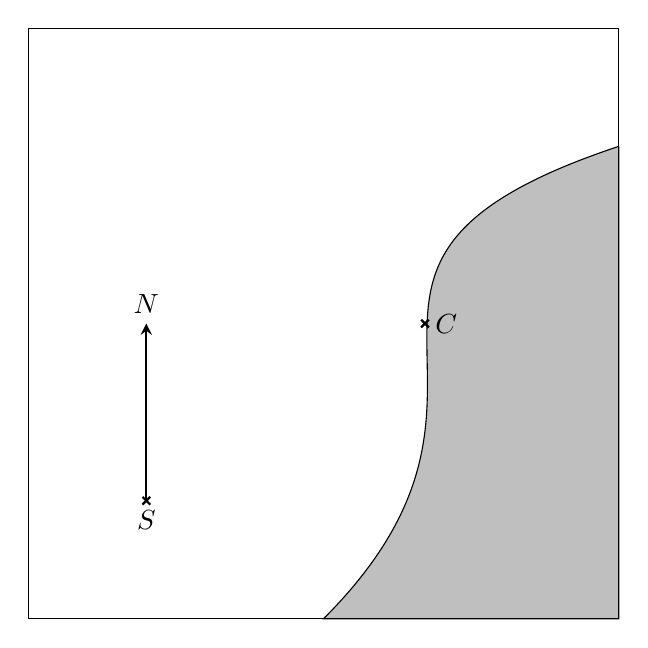
\begin{tikzpicture}[scale=1.5]
      \tkzDefPoints{1/1/S, 1/2.5/N, 3.36/2.5/C, 10/3.5/L}
      \draw (0,0) -- (5,0) -- (5,5) -- (0,5) -- (0,0); 
      \filldraw[fill=gray!50] (5,4) .. controls (2,3) and (4.5, 2) .. (2.5,0) -- (5,0) -- (5,4);
      \tkzDrawPoint[shape=cross out,thick](S)
      \tkzDrawPoint[shape=cross out,thick](C)
      \tkzDrawSegment[-stealth, thick](S,N)

      \tkzLabelPoints[below](S)
      \tkzLabelPoints[above](N)
      \tkzLabelPoints[right](C)
    \end{tikzpicture}
  \end{figure}
  Scale	1 cm represents 100 m.\\
  Point $C$ is on the coast. Ships must not sail closer than $500$ m to point $C$.\\
  The ship sails on a bearing of 0\ang{37}\\
  Will the ship sail closer than 500 m to point $C$?\\
  You must explain your answer.\strch




  




\end{enumerate}
  % 
\chapter{Congruent Triangle Proofs}

\begin{enumerate}
  \item \mrk{4}
  \begin{figure}[H]
    \centering
    \begin{tikzpicture}[scale=1.3]
      \tkzDefPoints{0/4/A,-5/0/B,3/0/C,5/1.8/L}
      \tkzDrawPolygon(A,B,C)

      \tkzDefMidPoint(A,B) \tkzGetPoint{L}
      \tkzDefMidPoint(A,C) \tkzGetPoint{M}
      \tkzDefMidPoint(B,C) \tkzGetPoint{N}

      \tkzDrawSegments(L,M M,N)

      \tkzLabelPoint[above](A){A}
      \tkzLabelPoints[left](B, L)
      \tkzLabelPoint[right](C, M)
      \tkzLabelPoint[below](N){N}
    \end{tikzpicture}
  \end{figure}
\end{enumerate}
  % 
\chapter{GCSE Revision: Functions and Function Transformation Questions}

\begin{enumerate}
  \item \mrk{3}
  \begin{figure}[H]
    \centering
    \textbf{A}
    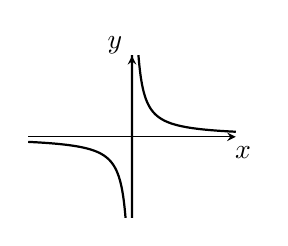
\begin{tikzpicture}
      \begin{axis}[
          xmin = -8, xmax = 8,
          ymin = -8, ymax = 8,
          xticklabels = {},
          yticklabels = {},
          xtick = {0},
          ytick = {0},
          axis lines = middle,
          height = 0.3\textwidth,
          x label style={at={(ticklabel* cs:0.95)},anchor=north west},
          y label style={at={(ticklabel* cs:0.95)},anchor=south east},
          xlabel = {$x$},
          ylabel = {$y$},
        ]
        % Plot a function
        \addplot[
          domain = -8:8,
          samples = 200,
          smooth,
          thick,
        ] {4/x};
      \end{axis}
    \end{tikzpicture}
    \hspace*{1cm}
    \textbf{B}
    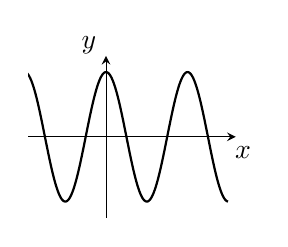
\begin{tikzpicture}
      \begin{axis}[
          xmin = -6, xmax = 10,
          ymin = -5, ymax = 5,
          xticklabels = {},
          yticklabels = {},
          xtick = {0},
          ytick = {0},
          axis lines = middle,
          height = 0.3\textwidth,
          x label style={at={(ticklabel* cs:0.95)},anchor=north west},
          y label style={at={(ticklabel* cs:0.95)},anchor=south east},
          xlabel = {$x$},
          ylabel = {$y$},
        ]
        % Plot a function
        \addplot[
          domain = -6.4:9.4,
          samples = 200,
          smooth,
          thick,
        ] {4*cos(deg(x))};
      \end{axis}
    \end{tikzpicture}\par
    \textbf{C}
    \begin{tikzpicture}
      \begin{axis}[
          xmin = -2, xmax = 1.5,
          ymin = -2, ymax = 6,
          xticklabels = {},
          yticklabels = {},
          xtick = {0},
          ytick = {0},
          axis lines = middle,
          height = 0.3\textwidth,
          x label style={at={(ticklabel* cs:0.95)},anchor=north west},
          y label style={at={(ticklabel* cs:0.95)},anchor=south east},
          xlabel = {$x$},
          ylabel = {$y$},
        ]
        % Plot a function
        \addplot[
          domain = -2:1,
          samples = 200,
          smooth,
          thick,
        ] {4*2^x};
      \end{axis}
    \end{tikzpicture}
    \hspace*{1cm}
    \textbf{D}
    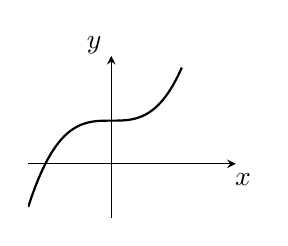
\begin{tikzpicture}
      \begin{axis}[
          xmin = -2, xmax = 3,
          ymin = -5, ymax = 10,
          xticklabels = {},
          yticklabels = {},
          xtick = {0},
          ytick = {0},
          axis lines = middle,
          height = 0.3\textwidth,
          x label style={at={(ticklabel* cs:0.95)},anchor=north west},
          y label style={at={(ticklabel* cs:0.95)},anchor=south east},
          xlabel = {$x$},
          ylabel = {$y$},
        ]
        % Plot a function
        \addplot[
          domain = -2:1.7,
          samples = 200,
          smooth,
          thick,
        ] {x^3+4};
      \end{axis}
    \end{tikzpicture}\par
    \textbf{E}
    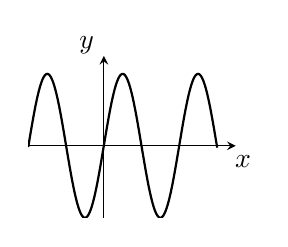
\begin{tikzpicture}
      \begin{axis}[
          xmin = -6.3, xmax = 11,
          ymin = -4, ymax = 5,
          xticklabels = {},
          yticklabels = {},
          xtick = {0},
          ytick = {0},
          axis lines = middle,
          height = 0.3\textwidth,
          x label style={at={(ticklabel* cs:0.95)},anchor=north west},
          y label style={at={(ticklabel* cs:0.95)},anchor=south east},
          xlabel = {$x$},
          ylabel = {$y$},
        ]
        % Plot a function
        \addplot[
          domain = -6.3:9.45,
          samples = 200,
          smooth,
          thick,
        ] {4*sin(deg(x))};
      \end{axis}
    \end{tikzpicture}
    \hspace*{1cm}
    \textbf{F}
    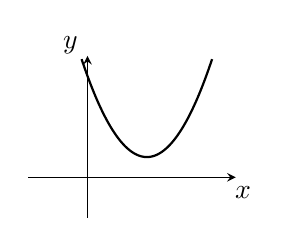
\begin{tikzpicture}
      \begin{axis}[
          xmin = -2, xmax = 5,
          ymin = -2, ymax = 6,
          xticklabels = {},
          yticklabels = {},
          xtick = {0},
          ytick = {0},
          axis lines = middle,
          height = 0.3\textwidth,
          x label style={at={(ticklabel* cs:0.95)},anchor=north west},
          y label style={at={(ticklabel* cs:0.95)},anchor=south east},
          xlabel = {$x$},
          ylabel = {$y$},
        ]
        % Plot a function
        \addplot[
          domain = -0.2:4.2,
          samples = 200,
          smooth,
          thick,
        ] {x^2-4*x+5};
      \end{axis}
    \end{tikzpicture}
  \end{figure}
  Each equation in the table represents one of the graphs \textbf{A} to \textbf{F}.\\
  Write the letter of each graph in the correct place in the table.
  \begin{table}[H]
    \centering
    \begin{tabular}{| l | l |} 
      \hline
      \textbf{Equation} & \textbf{Graph} \\
      \hline
      $y = 4\sin x^\circ$ &  \\ 
      \hline
      $y = 4\cos x^\circ$ &  \\
      \hline
      $y = x^2 - 4x + 5$ & \\
      \hline
      $y = 4 \times 2^x$ & \\
      \hline
      $y = x^3 + 4$ & \\
      \hline
    \end{tabular}
  \end{table}
  \item \mbox{}
  \begin{enumerate}
    \begin{figure}[H]
      \centering
      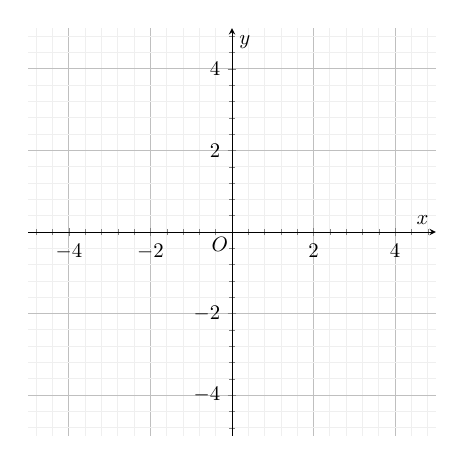
\begin{tikzpicture}[scale=0.75]
        \begin{axis}[
            xmin = -5, xmax = 5,
            ymin = -5, ymax = 5,
            grid = both,
            minor tick num = 4,
            major grid style = {lightgray},
            minor grid style = {lightgray!25},
            axis lines = middle,
            width = 0.7\textwidth,
            height = 0.7\textwidth,
            xlabel = {$x$},
            ylabel = {$y$},
          ]
          \node at (-0.3, -0.3) {$O$};
        \end{axis}
      \end{tikzpicture}
    \end{figure}
    \item On the grid, draw the graph of $x^2 + y^2 = 4$.\mrk{2}
    \begin{figure}[H]
      \centering
      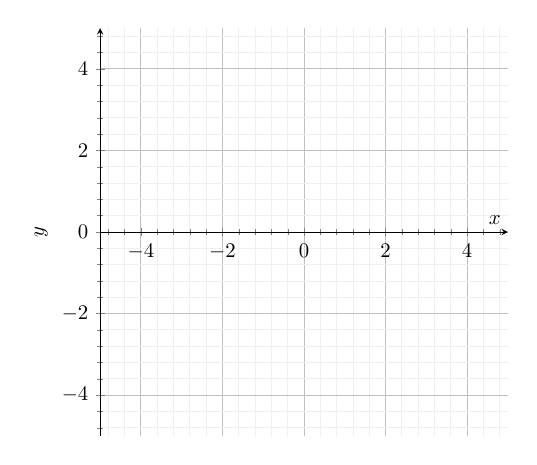
\begin{tikzpicture}[scale=0.75]
        \begin{axis}[
            xmin = -5, xmax = 5,
            ymin = -5, ymax = 5,
            grid = both,
            minor tick num = 4,
            major grid style = {lightgray},
            minor grid style = {lightgray!25},
            axis y line = left, 
            axis x line = middle,
            width = 0.7\textwidth,
            height = 0.7\textwidth,
            xlabel = {$x$},
            ylabel = {$y$},
          ]
          \end{axis}
        \end{tikzpicture}
      \end{figure}
      \item On the grid, sketch the graph of $y = \cos x$ for $\ang{0} \leq x \leq \ang{360}$.\mrk{2}
  \end{enumerate}
  \item %
  \begin{enumerate}
    \item Complete the table of values for $y = x^3 - 7$.\mrk{2}
    \begin{table}[H]
      \centering
      \begin{tabular}{|m{1cm}|m{1cm}|m{1cm}|m{1cm}|m{1cm}|m{1cm}|m{1cm}|} 
        \hline
        $x$ &	-2 & -1 &	0 &	1 &	2 &	3 \\
        \hline
        $y$ & -8 & & & & & 20 \\
        \hline
      \end{tabular}
    \end{table}
    \item On the grid, draw the graph of $y = x^3 - 7$ for values of $x$ from $-2$ to $3$.\mrk{2}
    \begin{figure}[H]
      \centering
      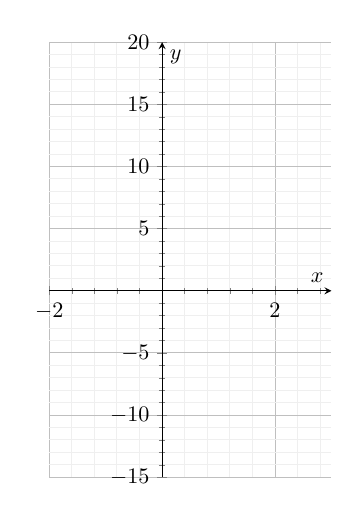
\begin{tikzpicture}[scale=0.8]
        \begin{axis}[
            xmin = -2, xmax = 3,
            ymin = -15, ymax = 20,
            grid = both,
            minor tick num = 4,
            major grid style = {lightgray},
            minor grid style = {lightgray!25},
            axis lines = middle,
            width = 0.5\textwidth,
            height = 0.7\textwidth,
            xlabel = {$x$},
            ylabel = {$y$},
          ]
          \end{axis}
        \end{tikzpicture}
      \end{figure}
  \end{enumerate}
  \item %
  \begin{enumerate}
    \item Construct the graph of $x^2 + y^2 = 9$.
    \begin{figure}[H]
      \centering
      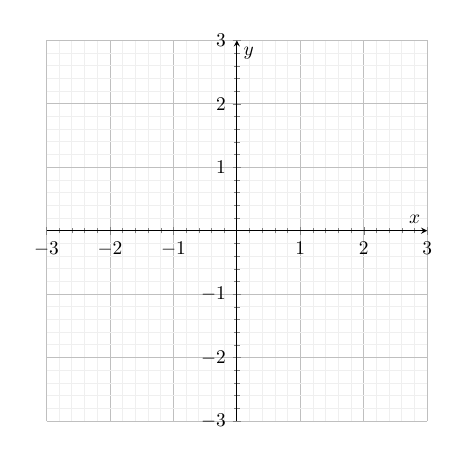
\begin{tikzpicture}[scale=0.7]
        \begin{axis}[
            xmin = -3, xmax = 3,
            ymin = -3, ymax = 3,
            grid = both,
            minor tick num = 4,
            major grid style = {lightgray},
            minor grid style = {lightgray!25},
            axis lines = middle,
            width = 0.7\textwidth,
            height = 0.7\textwidth,
            xlabel = {$x$},
            ylabel = {$y$},
          ]
          \end{axis}
        \end{tikzpicture}
      \end{figure}
      \item By drawing the line $x + y = 1$ on the grid, solve the equations
      \begin{align*}
        x^2 + y^2 &= 9\\
        x + y &= 1
      \end{align*}
  \end{enumerate}
  \item %
  \begin{enumerate}
    \item Complete the table of values for $y = x^2 + x - 3$.\mrk{2}
    \begin{table}[H]
      \centering
      \begin{tabular}{|m{1cm}|m{1cm}|m{1cm}|m{1cm}|m{1cm}|m{1cm}|m{1cm}|m{1cm}|} 
        \hline
        $x$	& -4 & -3 & -2 & -1 &	0 &	1 &	2 \\
        \hline
        $y$ & 9 & & -1 & -3 & & & 3 \\
        \hline
      \end{tabular}
    \end{table}
    \item On the grid below, draw the graph of $y = x^2 + x - 3$ for values of $x$ from $-4$ to $2$.\mrk{2}
    \begin{figure}[H]
      \centering
      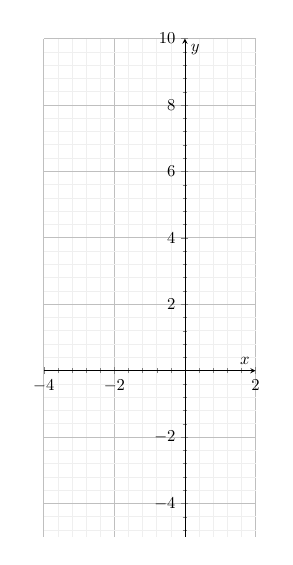
\begin{tikzpicture}[scale=0.6]
        \begin{axis}[
            xmin = -4, xmax = 2,
            ymin = -5, ymax = 10,
            grid = both,
            minor tick num = 4,
            major grid style = {lightgray},
            minor grid style = {lightgray!25},
            axis lines = middle,
            width = 0.5\textwidth,
            height = \textwidth,
            xlabel = {$x$},
            ylabel = {$y$},
          ]
          \end{axis}
        \end{tikzpicture}
      \end{figure}
  \end{enumerate}
  \item The graph of $y = f(x)$ is shown on each of the grids.
  \begin{enumerate}
    \item On this grid, sketch the graph of $y = f(x - 3)$.\mrk{2}
    \begin{figure}[H]
      \centering
      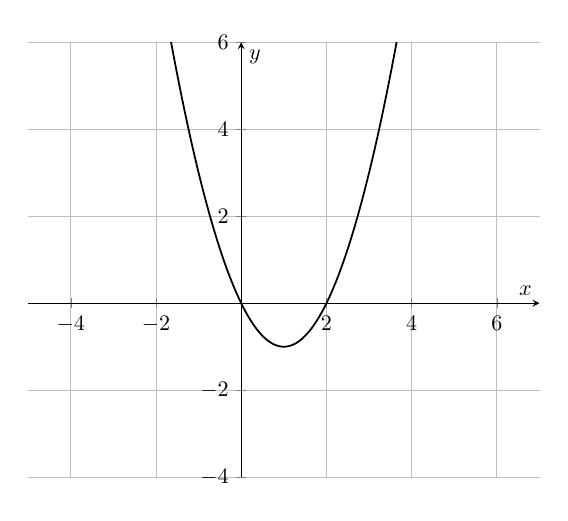
\begin{tikzpicture}[scale=0.8]
        \begin{axis}[
            xmin = -5, xmax = 7,
            ymin = -4, ymax = 6,
            grid = both,
            axis lines = middle,
            width = 0.8\textwidth,
            height = 0.7\textwidth,
            xlabel = {$x$},
            ylabel = {$y$},
          ]
          % Plot a function
          \addplot[
            domain = -2:4,
            samples = 200,
            smooth,
            thick,
          ] {x^2 - 2*x};
          \end{axis}
        \end{tikzpicture}
      \end{figure}
      \item On this grid, sketch the graph of $y = 2f(x)$.\mrk{2}
      \begin{figure}[H]
        \centering
        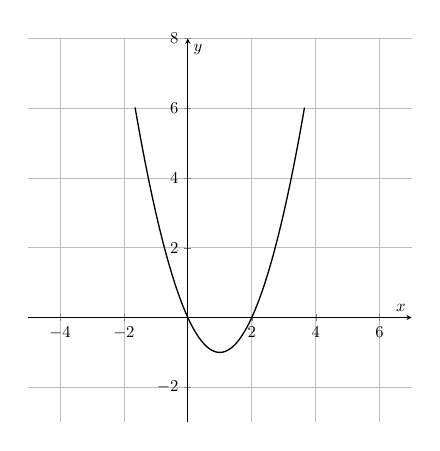
\begin{tikzpicture}[scale=0.6]
          \begin{axis}[
              xmin = -5, xmax = 7,
              ymin = -3, ymax = 8,
              grid = both,
              axis lines = middle,
              width = 0.8\textwidth,
              height = 0.8\textwidth,
              xlabel = {$x$},
              ylabel = {$y$},
            ]
            % Plot a function
            \addplot[
              domain = -1.65:3.65,
              samples = 200,
              smooth,
              thick,
            ] {x^2 - 2*x};
            \end{axis}
          \end{tikzpicture}
        \end{figure}
  \end{enumerate}
  \item The graph of $y = f(x)$ is shown on the grids.
  \begin{enumerate}
    \item On this grid, sketch the graph of $y = f(x - 3)$.\mrk{2}
  \end{enumerate}
  

\end{enumerate}
  % 
\chapter{GCSE Revision - Loci and Constructions}

\begin{enumerate}
  \item Draw the locus of all points which are equidistant from the lines $AB$ and $AC$.\mrk{2}
  \begin{figure}[H]
    \centering
    \begin{tikzpicture}
      \tkzDefPoints{0/0/A,0/4/B,5/0/C}
      \tkzDrawSegments(A,B A,C)
      \tkzLabelPoints[above,left](B)
      \tkzLabelPoints[below,left](A)
      \tkzLabelPoints[below,right](C)
    \end{tikzpicture}
  \end{figure}
  \item Use ruler and compasses to \textbf{construct} the perpendicular bisector of the line $AB$. You must show all your construction line.\mrk{2}\strch
  \begin{figure}[H]
    \centering
    \begin{tikzpicture}
      \tkzDefPoints{0/0/A,6/0/B}
      \tkzDrawSegments(A,B)
      \tkzLabelPoints[below,left](A)
      \tkzLabelPoints[below,right](B)
    \end{tikzpicture}
  \end{figure}
  \newpage
  \item Use ruler and compasses to \textbf{construct} an angle of $\ang{30}$ at $P$. You must show all your construction lines.\mrk{3}\strch
  \begin{figure}[H]
    \centering
    \begin{tikzpicture}
      \tkzDefPoints{0/0/P,6/0/B}
      \tkzDrawSegments(P,B)
      \tkzLabelPoints[below,left](P)
    \end{tikzpicture}
  \end{figure}
  \item Here is a map.\\
  The map shows two towns, Burford and Hightown
  \begin{figure}[H]
    \centering
    \begin{tikzpicture}
      \tkzDefPoints{0/0/A,10/0/B, 3/7.5/m1, 8/2.5/m2}
      \tkzDefSquare(A,B)\tkzGetPoints{C}{D}
      \tkzDrawPolygon(A,B,C,D)
      \tkzDrawPoints[shape=cross out, size=8pt](m1,m2)
      \tkzLabelPoint[above=3pt](m1){Burford}
      \tkzLabelPoint[below=3pt](m2){Hightown}
    \end{tikzpicture}
  \end{figure}
  Scale: 1 cm represents 10 km.\par 
  A company is going to build a warehouse. The warehouse will be less than $30$ km from Burford and less than $50$ km from Hightown. Shade the region on the map where the company can build the warehouse.\mrk{3}
  \newpage
  \item Here is a scale drawing of a rectangular garden $ABCD$.\mrk{4}
  \begin{figure}[H]
    \centering
    \begin{tikzpicture}[scale=1.2]
      \tkzDefPoints{0/0/A,10/0/B, 10/-7/C}

      \tkzDefParallelogram(A,B,C)
      \tkzGetPoint{D}

      \tkzDrawPolygon(A,B,C,D)


      \tkzLabelPoints[above,left](A)
      \tkzLabelPoints[above,right](B)
      \tkzLabelPoints[below,right](C)
      \tkzLabelPoints[below,left](D)
    \end{tikzpicture}
  \end{figure}
  Scale: 1 cm represents 1 metre.\par 
  Jane wants to plant a tree in the garden at least 5m from point $C$, nearer to $AB$ than to $AD$, and less than 3m from $DC$.\\
  On the diagram, shade the region where Jane can plant the tree.
\end{enumerate}
  % 
\chapter{GCSE Revision - Number Questions}
Standard Form, Bounds, Percentages, Direct/Indirect Proportion, Fractions, Line Graphs, LCM.

\begin{enumerate}
  \item %
  \begin{enumerate}
    \item Write $7.8 \time 10^{-4}$ as an ordinary number.\mrk{1}\\[2cm]\vspace*{0pt}\hfill\dline
    \item Write $95 600 000$ as a number in standard form.\mrk{1}\\[2cm]\vspace*{0pt}\hfill\dline
  \end{enumerate}
  \lmrk{1}{2}
  \item In a sale normal prices are reduced by $20\%$. A washing machine has a sale price of $\pounds 464$. By how much money is the normal price of the washing machine reduced?\mrk{3}\\[4cm]\vspace*{0pt}\hfill\pounds\dline
  \item $y$ is directly proportional to the square of $x$. When $x = 3,\ y = 36$. Find the value of $y$ when $x = 5$.\mrk{4}\\[2cm]\vspace*{0pt}\hfill\dline
  \item %
  $$
  m = \frac{\sqrt{s}}{t}
  $$
  $s = 3.47$ correct to $2$ decimal places.\\
  $t = 8.132$ correct to $3$ decimal places.\par 
  By considering bounds, work out the value of $m$ to a suitable degree of accuracy. You must show all your working and give a reason for your final answer.\\[3cm]\vspace*{0pt}
  \item %
  \begin{enumerate}
    \item Write $8.2 \times 10^5$ as an ordinary number.\mrk{1}\\[1.5cm]\vspace*{0pt}\hfill\dline
    \item Write $0.000376$ in standard form.\mrk{1}\\[1.5cm]\vspace*{0pt}\hfill\dline
    \item Work out the value of $(2.3 \times 10^{12}) \divisionsymbol (4.6 \times 10^3)$. Give your answer in standard form.\mrk{2}\\[2cm]\vspace*{0pt}\hfill\dline
  \end{enumerate}
  \lmrk{5}{4}
  \item $h$ is inversely proportional to the square of $r$. When $r = 5,\ h = 3.4$. Find the value of $h$ when $r = 8$.\mrk{3}\\[2.5cm]\vspace*{0pt}\hfill$h=$\dline
  \item Dan does an experiment to find the value of $\pi$. He measures the circumference and the diameter of a circle. He measures the circumference, $C$, as $170$ mm to the nearest millimetre. He measures the diameter, $d$, as $54$ mm to the nearest millimetre.\par 
  Dan uses $\pi = \dfrac{C}{d}$ to find the value of $\pi$. Calculate the upper bound and the lower bound for Dan's value of $\pi$.\mrk{4}\\[3cm]
  \vspace*{0pt}\hfill upper bound = \dline\\
  \vspace*{0pt}\hfill lower bound = \dline
  \item Viv wants to invest $\pounds 2000$ for $2$ years in the same bank.\\[0.5cm]
  \fbox{\parbox[c]{0.4\textwidth}{\centering
		\textbf{The International Bank}\\[0.5cm]
    Compound Interest\\[0.5cm]
    $4\%$ for the first year\\
    $1\%$ for each extra year}}\hfill
    \fbox{\parbox[c]{0.4\textwidth}{\centering
		\textbf{The Friendly Bank}\\[0.5cm]
    Compound Interest\\[0.5cm]
    $5\%$ for the first year\\
    $0.5\%$ for each extra year}}\\[0.5cm]
    At the end of 2 years, Viv wants to have as much money as possible. Which bank should she invest her $\pounds 2000$ in?\mrk{4}
    \newpage
    \item One sheet of paper is $9 \times 10^{-3}$ cm thick. Mark wants to put 500 sheets of paper into the paper tray of his printer. The paper tray is $4$ cm deep.\par 
    Is the paper tray deep enough for 500 sheets of paper? You must explain your answer.\mrk{3}\\[2cm]\vspace*{0pt}
    \item The normal price of a television is reduced by $30\%$ in a sale. The sale price of the television is $\pounds 350$ Work out the normal price of the television.\mrk{3}\\[2cm]\vspace*{0pt}\hfill$\pounds$ \dline
    \item Write the following numbers in order of size. Start with the smallest number.\mrk{2}
    $$
    0.038 \times 10^2 \qquad 3800 \times 10^{-4} \qquad 380 \qquad 0.38 \times 10^{-1}
    $$\\[2cm]\vspace*{0pt}
    \item Talil is going to make some concrete mix. He needs to mix cement, sand and gravel in the ratio $1 : 3 : 5$ by weight.\par
    Talil wants to make 180 kg of concrete mix. Talil has\par 
    \hspace*{1cm} 15 kg of cement\\
    \hspace*{1cm} 85 kg of sand\\
    \hspace*{1cm} 100 kg of gravel\par
    Does Talil have enough cement, sand and gravel to make the concrete mix?\mrk{4}
    \newpage
    \item Work out an estimate for $\dfrac{31\times 9.87}{0.509}$.\mrk{3}\\[2cm]\vspace*{0pt}
    \item The average fuel consumption ($c$) of a car, in kilometres per litre, is given by the formula
    $$
    c = \frac{d}{f}
    $$
    where $d$ is the distance travelled, in kilometres, and $f$ is the fuel used, in litres.\par 
    d = 163 correct to 3 significant figures.\\
    f = 45.3 correct to 3 significant figures.\par 
    By considering bounds, work out the value of $c$ to a suitable degree of accuracy. You must show all of your working and give a reason for your final answer.\mrk{5}\\[3cm]\vspace*{0pt}\hfill$c=$ \dline
    \item %
    \begin{enumerate}
      \item Write $6.43 \times 10^5$ as an ordinary number.\mrk{1}\\[1cm]\vspace*{0pt}\hfill\dline
      \item Work out the value of $2 \times 10^7 \times 8 \times 10^{-12}$ Give your answer in standard form.\mrk{2}\\[2cm]\vspace*{0pt}\hfill\dline
    \end{enumerate}
    \item %
    $$
    p^2 = \frac{x-y}{xy}
    $$
    $x = 8.5 \times 10^9$\\
    $y = 4 \times 10^8$\par 
    Find the value of $p$. Give your answer in standard form correct to 2 significant figures.\mrk{3}\\[3cm]\vspace*{0pt}\hfill\dline
    \item Liam invests $\pounds 6200$ for $3$ years in a savings account. He gets $2.5\%$ per annum compound interest.\par
    How much money will Liam have in his savings account at the end of $3$ years?\mrk{3}\\[3cm]\vspace*{0pt}\hfill$\pounds$\dline
    \item Express the recurring decimal $0.2\dot{8}\dot{1}$ as a fraction in its simplest form.\mrk{3}\\[2cm]\vspace*{0pt}\hfill\dline
    \item %
    \begin{enumerate}
      \item Write down the value of $10^0$.\mrk{1}\\\vspace*{0pt}\hfill\dline
      \item Write $6.7 \times 10^{-5}$ as an ordinary number.\mrk{1}\\\vspace*{0pt}\hfill\dline
      \item Work out the value of $(3 \times 10^7) \times (9 \times 10^6)$. Give your answer in standard form.\mrk{2}\\[2cm]\vspace*{0pt}\hfill\dline
    \end{enumerate}
    \lmrk{19}{4}
    \item %
    \begin{enumerate}
      \item Work out the value of $(6 \times 108) \times (4 \times 10^7)$. Give your answer in standard form.\mrk{2}\\[1.5cm]\vspace*{0pt}\hfill\dline
      \item Work out the value of $(6 \times 10^8) + (4 \times 10^7)$. Give your answer in standard form.\mrk{2}\\[1.5cm]\vspace*{0pt}\hfill\dline            
    \end{enumerate}
    \newpage
    \item Use your calculator to work out
    $$
    \sqrt{\frac{921 - 170\tan \ang{65}}{0.012 + 0.034}}
    $$
    \begin{enumerate}
      \item Write down all the figures on your calculator display. You must write your answer as a decimal.\mrk{2}\\[1.5cm]\vspace*{0pt}\hfill\dline    
    \end{enumerate}
    \item %
    \begin{enumerate}
      \item Write $82 500 000$ in standard form.\mrk{1}\\[1.5cm]\vspace*{0pt}\hfill\dline
      \item Work out $(5.2 \times 10^{-7}) \times (2.8 \times 10^{-9})$. Give your answer in standard form.\mrk{2}\\[1.5cm]\vspace*{0pt}\hfill\dline    
    \end{enumerate}
    \item $P$ is inversely proportional to $V$. When $V = 8,\ P = 5$
    \begin{enumerate}
      \item Find a formula for $P$ in terms of $V$.\mrk{3}\\[2cm]\vspace*{0pt}\hfill\dline
      \item Calculate the value of $P$ when $V = 2$.\mrk{1}\\[2cm]\vspace*{0pt}\hfill\dline
    \end{enumerate}
    \item Work out $1.83 \times 47$.
    \newpage
    \item You can use this conversion graph to change between pounds (\pounds) and dollars (\$).
    \begin{figure}[H]
      \centering
      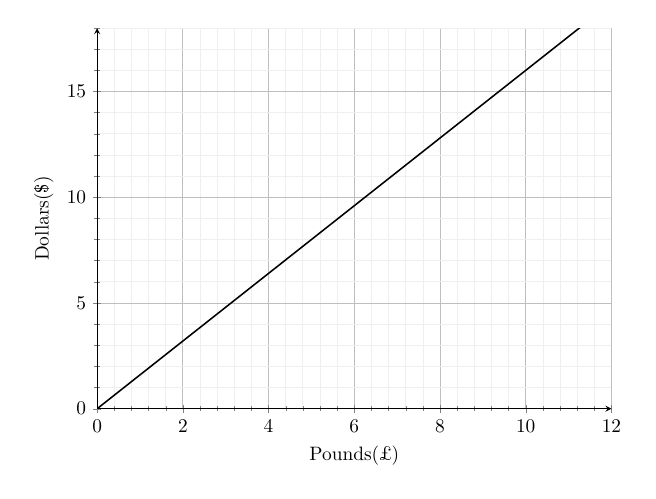
\begin{tikzpicture}[scale=0.7]
        \begin{axis}[
            xmin = 0, xmax = 12,
            ymin = 0, ymax = 18,
            grid = both,
            minor tick num = 4,
            major grid style = {lightgray},
            minor grid style = {lightgray!25},
            axis lines = left,
            width = 0.9\textwidth,
            height = 0.7\textwidth,
            xlabel = {Pounds(\pounds)},
            ylabel = {Dollars(\$)},
          ]
          % Plot a function
          \addplot[
            domain = 0:12,
            samples = 200,
            smooth,
            thick,
          ] {8/5*x};
          \end{axis}
        \end{tikzpicture}
      \end{figure}
      \begin{enumerate}
        \item Use the conversion graph to change $\pounds 5$ to dollars.\mrk{1}\\[1cm]\vspace*{0pt}\hfill\$\dline\\
        Ella has \$200 and \pounds 800. Her hotel bill is \$600. Ella pays the bill with the \$200 and some of the pounds
        \item Use the conversion graph to work out how many pounds she has left.\mrk{4}\\[1cm]\vspace*{0pt}\hfill\pounds\dline
      \end{enumerate}
      \lmrk{25}{4}
      \item Trams leave Piccadilly\par
      \hspace*{2cm} to Eccles every 9 minutes \hspace*{2cm} to Didsbury every 12 minutes\par
      A tram to Eccles and a tram to Didsbury both leave Piccadilly at 9 a.m. At what time will a tram to Eccles  and a tram to Didsbury next leave Piccadilly at the same time?\mrk{3}\\[2cm]\vspace*{0pt}\hfill\dline
      \item Given that	$1793 \times 185 = 331 705$. Write down the value of
      \begin{enumerate}
        \item $1.793 \times 185$\\\vspace*{0pt}\hfill\dline
        \item $331 705 \divisionsymbol 1.85$\\\vspace*{0pt}\hfill\dline
      \end{enumerate}
      \lmrk{27}{2}
      \item Write $525$ as a product of its prime factors.\mrk{3}\\[3cm]\vspace*{0pt}\hfill\dline
      \item Ed has 4 cards. There is a number on each card.      
      \begin{figure}[H]
        \centering
        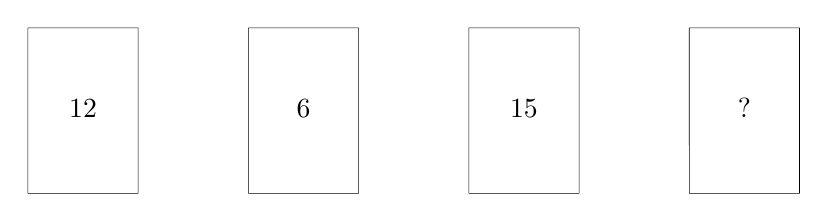
\begin{tikzpicture}[scale=0.7]
          \tkzDefPoints{0/0/a1,2/0/b1,2/3/c1}
          \tkzDefPoints{4/0/a2,6/0/b2,6/3/c2}
          \tkzDefPoints{8/0/a3,10/0/b3,10/3/c3}
          \tkzDefPoints{12/0/a4,14/0/b4,14/3/c4}

          \tkzDefParallelogram(a1,b1,c1)
          \tkzGetPoint{d1}

          \tkzDefParallelogram(a2,b2,c2)
          \tkzGetPoint{d2}

          \tkzDefParallelogram(a3,b3,c3)
          \tkzGetPoint{d3}

          \tkzDefParallelogram(a4,b4,c4)
          \tkzGetPoint{d4}

          \tkzDrawPolygon(a1,b1,c1,d1)
          \tkzDrawPolygon(a2,b2,c2,d2)
          \tkzDrawPolygon(a3,b3,c3,d3)
          \tkzDrawPolygon(a4,b4,c4,d4)

          \tkzDefMidPoint(a1,c1)
          \tkzGetPoint{l1}

          \tkzDefMidPoint(a2,c2)
          \tkzGetPoint{l2}

          \tkzDefMidPoint(a3,c3)
          \tkzGetPoint{l3}

          \tkzDefMidPoint(a4,c4)
          \tkzGetPoint{l4}

          \tkzLabelPoint[above=-6pt](l1){12}
          \tkzLabelPoint[above=-6pt](l2){6}
          \tkzLabelPoint[above=-6pt](l3){15}
          \tkzLabelPoint[above=-6pt](l4){?}
        \end{tikzpicture}
      \end{figure}
      The mean of the 4 numbers on Ed's cards is 10. Work out the number on the 4th card.\mrk{3}\\[3cm]\vspace*{0pt}\hfill\dline
      \item Here are the ingredients needed to make 12 shortcakes.
      \begin{center}
        \fbox{\parbox[c]{0.4\textwidth}{\centering
          \textbf{Shortcakes}\\[0.3cm]
          Makes \textbf{12} shortcakes\\[0.2cm]
          50 g 	of sugar\\
          200 g of butter\\
          200 g of flour\\
          10 ml of milk}}
      \end{center}
      Liz makes some shortcakes. She uses 25 ml of milk.
      \begin{enumerate}
        \item How many shortcakes does Liz make?\mrk{2}\\[2cm]\vspace*{0pt}\hfill\dline\\
        Robert has \par
        \hspace*{2cm}500 g of sugar\\
			  \hspace*{2cm}1000 g of butter\\
			  \hspace*{2cm}1000 g of flour\\
			  \hspace*{2cm}500 ml of milk
        \item Work out the greatest number of shortcakes Robert can make.\mrk{2}\\[2cm]\vspace*{0pt}\hfill\dline
      \end{enumerate}
      \lmrk{30}{4}
      \item Buses to Acton leave a bus station every 24 minutes. Buses to Barton leave the same bus station every 20 minutes. A bus to Acton and a bus to Barton both leave the bus station at 9:00 am.\par 
      When will a bus to Acton and a bus to Barton next leave the bus station at the same time?\mrk{3}\\[3cm]\vspace*{0pt}\hfill\dline
      \item Work out an estimate for the value of $(0.49 \times 0.61)^2$.\mrk{2}\\[2cm]\vspace*{0pt}\hfill\dline
      \newpage
      \item %
      \begin{enumerate}
        \item Work out $\dfrac{2}{3} \divisionsymbol \dfrac{5}{6}$. Give your fraction in its simplest form.\mrk{3}\\[2.5cm]\vspace*{0pt}\hfill\dline
        \item Work out $2\dfrac{1}{3} - 1\dfrac{2}{5}$.\mrk{3}\\[2.5cm]\vspace*{0pt}\hfill\dline
      \end{enumerate}
      \lmrk{33}{6}
      \item %
      \begin{enumerate}
        \item Work out $2\dfrac{17}{20} - 1\dfrac{2}{5}$.\mrk{3}\\[2.5cm]\vspace*{0pt}\hfill\dline
        \item Work out $2\dfrac{2}{3} \times 1\dfrac{3}{4}$.\mrk{3}\\[2.5cm]\vspace*{0pt}\hfill\dline
      \end{enumerate}
      \lmrk{34}{6}
      \item Work out $3\dfrac{1}{4} \times 2\dfrac{2}{3}$. Give your answer in its simplest form.\mrk{3}\\[2.5cm]\vspace*{0pt}\hfill\dline
      \item The diagram shows the floor of a village hall.
      \begin{figure}[H]
        \centering
        \begin{tikzpicture}
          \tkzDefPoints{0/0/a,4/0/b,4/-1.5/c,6/-1.5/d,6/-3.5/e,0/-3.5/f, 9/-0.5/L}

          \tkzDrawPolygon(a,b,c,d,e,f)

          \tkzLabelSegment(a,b){9m}
          \tkzLabelSegment(d,e){6m}
          \tkzLabelSegment(e,f){16m}
          \tkzLabelSegment(f,a){8m}

          \tkzMarkRightAngles(a,b,c c,d,e d,e,f e,f,a f,a,b)

          \tkzLabelPoint[above](L){Diagram \textbf{NOT}}
          \tkzLabelPoint[below](L){accurately drawn}
        \end{tikzpicture}
      \end{figure}
      The caretaker needs to polish the floor.\par
      One tin of polish normally costs $\pounds 19$.\\
      One tin of polish covers $12$ $m^2$ of floor.\par
      There is a discount of 30\% off the cost of the polish. The caretaker has $\pounds 130$.\par 
      Has the caretaker got enough money to buy the polish for the floor? You must show all your working.
\end{enumerate}
  % 
\chapter{GCSE Revision - Probability}

\begin{enumerate}
  \item In a supermarket, the probability that John buys fruit is 0.7. In the same supermarket, the probability that John independently buys vegetables is 0.4.\par 
  Work out the probability that John buys fruit or buys vegetables or buys both.\mrk{4}\\[3cm]\vspace*{0pt}\hfill\dline
  \item There are three different types of sandwiches on a shelf. There are 4 egg sandwiches, 5 cheese sandwiches and 2 ham sandwiches. Erin takes at random 2 of these sandwiches.\par 
  Work out the probability that she takes 2 different types of sandwiches.
  \newpage
  \item Fiza has 10 coins in a bag. There are three $\pounds 1$ coins and seven 50 pence coins. Fiza takes at random, 3 coins from the bag.\par
  Work out the probability that she takes exactly $\pounds 2.50$.
  \item Here are seven tiles.
  \begin{figure}[H]
    \centering
    \begin{tikzpicture}[scale=0.6]
      \tkzDefPoints{0/0/a1, 2/0/b1, 3/0/a2, 5/0/b2, 6/0/a3, 8/0/b3, 9/0/a4, 11/0/b4}
      \tkzDefPoints{12/0/a5, 14/0/b5, 15/0/a6, 17/0/b6, 18/0/a7, 20/0/b7}

      \tkzDefSquare(a1,b1) \tkzGetPoints{c1}{d1}
      \tkzDrawPolygon(a1,b1,c1,d1)

      \tkzDefSquare(a2,b2) \tkzGetPoints{c2}{d2}
      \tkzDrawPolygon(a2,b2,c2,d2)

      \tkzDefSquare(a3,b3) \tkzGetPoints{c3}{d3}
      \tkzDrawPolygon(a3,b3,c3,d3)

      \tkzDefSquare(a4,b4) \tkzGetPoints{c4}{d4}
      \tkzDrawPolygon(a4,b4,c4,d4)

      \tkzDefSquare(a5,b5) \tkzGetPoints{c5}{d5}
      \tkzDrawPolygon(a5,b5,c5,d5)

      \tkzDefSquare(a6,b6) \tkzGetPoints{c6}{d6}
      \tkzDrawPolygon(a6,b6,c6,d6)

      \tkzDefSquare(a7,b7) \tkzGetPoints{c7}{d7}
      \tkzDrawPolygon(a7,b7,c7,d7)

      \tkzDefMidPoint(a1,c1)
      \tkzGetPoint{l1}
      \tkzLabelPoint[above=-6pt](l1){1}

      \tkzDefMidPoint(a2,c2)
      \tkzGetPoint{l2}
      \tkzLabelPoint[above=-6pt](l2){1}

      \tkzDefMidPoint(a3,c3)
      \tkzGetPoint{l3}
      \tkzLabelPoint[above=-6pt](l3){2}

      \tkzDefMidPoint(a4,c4)
      \tkzGetPoint{l4}
      \tkzLabelPoint[above=-6pt](l4){2}

      \tkzDefMidPoint(a5,c5)
      \tkzGetPoint{l5}
      \tkzLabelPoint[above=-6pt](l5){2}

      \tkzDefMidPoint(a6,c6)
      \tkzGetPoint{l6}
      \tkzLabelPoint[above=-6pt](l6){3}

      \tkzDefMidPoint(a7,c7)
      \tkzGetPoint{l7}
      \tkzLabelPoint[above=-6pt](l7){3}
    \end{tikzpicture}
  \end{figure}
  Jim takes at random a tile.\\
  He does \textbf{not} replace the tile.\par 
  Jim then takes at random a second tile.
  \begin{enumerate}
    \item Calculate the probability that both the tiles Jim takes have the number $1$ on them.\mrk{2}\\[4cm]\vspace*{0pt}\hfill\dline
    \item Calculate the probability that the number on the second tile Jim takes is greater than the number on the first tile he takes.
  \end{enumerate}
  \newpage
  \item Carolyn has $20$ biscuits in a tin. She has\par 
  \hspace*{2cm}12 plain biscuits\\
	\hspace*{2cm}5 chocolate biscuits\\
	\hspace*{2cm}3 ginger biscuits\par
  Carolyn takes at random two biscuits from the tin. Work out the probability that the two biscuits were not the same type.\\[3cm]\mbox{}
  \item Jan has two boxes.\par
  There are 6 black and 4 white counters in box A.\\
  There are 7 black and 3 white counters in box B.\par
  Jan takes at random a counter from box A and puts it in box B.\\
  She then takes at random a counter from box B and puts it in box A.
  \begin{enumerate}
    \item Complete the probability tree diagram.\mrk{2}
    \begin{figure}[H]
      \centering
      \begin{tikzpicture}[line cap=round,line join=round,x=0.6cm,y=0.5cm]
        \coordinate (O) at (2,-1);
        \begin{scope}
         \node (A) at (9,2) {Black};
         \node (B) at (9,-4) {White};
         \node (C) at (16,4) {Black};
         \node (D) at (16,0) {White};
         \node (E) at (16,-2) {Black};
         \node (F) at (16,-6) {White}; 
        \end{scope}
        
        \draw (O) -- (A) -- (C)
                     (A) -- (D)
              (O) -- (B) -- (E)
                     (B) -- (F);
        \end{tikzpicture}
    \end{figure}
    \item Find the probability that after Jan has put the counter from box B into box A there will still be 6 black counters and 4 white counters in box A.\mrk{2}\strch\\\vspace*{0pt}\hfill\dline
  \end{enumerate}
  \item There are 5 red pens, 3 blue pens and 2 green pens in a box.\par
  Gary takes at random a pen from the box and gives the pen to his friend.\\
  Gary then takes at random another pen from the box.\par
  Work out the probability that both pens are the same color.\\[3cm]\mbox{}
  \item \mbox{}
  \begin{figure}[H]
    \centering
    \begin{tikzpicture}
      \tkzDefPoints{-1/2/A, 1/2/B, 0/0/C, -1.5/3/L1, 1.5/3/L2}
      \tkzDrawArc[black](C,A)(B)
      \tkzDrawSegments(A,L1 B,L2 L1,L2)

      \tkzDefShiftPoint[C](0:1.5){w1}
      \tkzDefShiftPoint[C](45:1.5){b1}
      \tkzDefShiftPoint[C](90:1.5){w2}
      \tkzDefShiftPoint[C](135:1.5){b2}
      \tkzDefShiftPoint[C](180:1.5){w3}
      \tkzDefShiftPoint[C](225:1.5){w4}
      \tkzDefShiftPoint[C](270:1.5){b3}
      \tkzDefShiftPoint[C](315:1.5){b4}

      \tkzDefShiftPoint[C](120:0.5){w5}
      \tkzDefShiftPoint[C](249:0.5){w6}
      \tkzDefShiftPoint[C](360:0.5){w7}

      \tkzDrawPoints[size=20, shape=circle, fill=none](w1,w2,w3,w4,b1,b2,b3,b4,w5,w6,w7)

      \tkzLabelPoint[above=-6.5pt](w1){W}
      \tkzLabelPoint[above=-6.5pt](w2){W}
      \tkzLabelPoint[above=-6.5pt](w3){W}
      \tkzLabelPoint[above=-6.5pt](w4){W}
      \tkzLabelPoint[above=-6.5pt](w5){W}
      \tkzLabelPoint[above=-6.5pt](w6){W}
      \tkzLabelPoint[above=-6.5pt](w7){W}

      \tkzLabelPoint[above=-6.5pt](b1){B}
      \tkzLabelPoint[above=-6.5pt](b2){B}
      \tkzLabelPoint[above=-6.5pt](b3){B}
      \tkzLabelPoint[above=-6.5pt](b4){B}
    \end{tikzpicture}
  \end{figure}
  There are 11 buttons in a bag.\par
  \hspace*{2cm}7 buttons are white.\\
	\hspace*{2cm}4 buttons are black.\par
  Harley takes a button at random from the bag, and keeps it.\\
  She now takes another button at random from the bag.\par
  Work out the probability that Harley takes a button of each color.
\end{enumerate}
  % 
\chapter{GCSE Questions - Right-Angled Triangles}

\begin{enumerate}
  \item $ABC$ is an isosceles triangle.
  \begin{figure}[H]
    \centering
    \begin{tikzpicture}[scale=0.8]
      \tkzDefPoints{0/0/B, 5/0/C, 2.5/6/A, 9/5/L}
  
      \tkzDrawPolygon(A,B,C)
      \tkzLabelPoints(C)
      \tkzLabelPoints[above](A)
      \tkzLabelPoints[below left](B)

      \tkzMarkAngles[size=1.2, mark=none](C,B,A A,C,B)
      \tkzLabelAngle[pos=0.8](C,B,A){$54^\circ$}
      \tkzLabelAngle[pos=0.8](A,C,B){$54^\circ$}

      \tkzLabelSegment[below](B,C){12 cm}

      \tkzLabelPoint[above](L){Diagram \textbf{NOT}}
      \tkzLabelPoint[below](L){accurately drawn}
    \end{tikzpicture}
  \end{figure}
  Work out the area of the triangle. Give your answer correct to 3 significant figures.\mrk{4}\strch\\\mbox{}\vspace*{0pt}\hfill\dline cm$^2$
  \newpage

  \item Here is a right-angled triangle.
  \begin{figure}[H]
    \centering
    \begin{tikzpicture}
      \tkzDefPoints{0/0/B, 6/0/C, 0/3.5/A, 8/3/L}
  
      \tkzDrawPolygon(A,B,C)
      \tkzLabelPoints(C)
      \tkzLabelPoints[above](A)
      \tkzLabelPoints[below](B)

      \tkzLabelSegment[below](B,C){70 cm}
      \tkzLabelSegment[left](A,B){39 cm}

      \tkzMarkRightAngles(C,B,A)

      \tkzLabelPoint[above](L){Diagram \textbf{NOT}}
      \tkzLabelPoint[below](L){accurately drawn}
    \end{tikzpicture}
  \end{figure}
  Work out the length of $AC$. Give your answer correct to 1 decimal place.\mrk{3}\\[3cm]\vspace*{0pt}\hfill\dline cm
  \item \mbox{}
  \begin{figure}[H]
    \centering
    \begin{tikzpicture}
      \tkzDefPoints{0/0/C, 6/0/B, 0/3.5/A, 8/3/L}
  
      \tkzDrawPolygon(A,B,C)
      \tkzLabelPoints[below](C)
      \tkzLabelPoints[above](A)
      \tkzLabelPoints(B)

      \tkzLabelSegment[left](A,C){6 cm}
      \tkzLabelSegment[above right=2pt](A,B){13 cm}

      \tkzMarkRightAngles(B,C,A)

      \tkzLabelPoint[above](L){Diagram \textbf{NOT}}
      \tkzLabelPoint[below](L){accurately drawn}
    \end{tikzpicture}
  \end{figure}
  ABC is a right-angled triangle.\\
  $AC = 6$ cm\\
  $AB = 13$ cm
  \begin{enumerate}
    \item Work out the length of $BC$. Give your answer correct to 3 significant figures.\mrk{3}\\[3cm]\vspace*{0pt}\hfill\dline cm
    \newpage
    \item \mbox{}
    \begin{figure}[H]
      \centering
      \begin{tikzpicture}
        \tkzDefPoints{0/0/R, 6/0/Q, 0/3.5/P, 8/3/L}
    
        \tkzDrawPolygon(P,Q,R)
        \tkzLabelPoints[below](R)
        \tkzLabelPoints[above](P)
        \tkzLabelPoints(Q)
  
        \tkzLabelSegment[left](P,R){17 cm}
        \tkzLabelSegment[above right=2pt](P,Q){25 cm}
  
        \tkzMarkRightAngles(Q,R,P)
  
        \tkzLabelPoint[above](L){Diagram \textbf{NOT}}
        \tkzLabelPoint[below](L){accurately drawn}
      \end{tikzpicture}
    \end{figure}
    PQR is a right-angled triangle.\\
    $R = 17$ cm\\
    $PQ = 25$ cm\\
    Work out the size of angle RPQ. Give your answer correct to 1 decimal place.\mrk{3}\\[3cm]\vspace*{0pt}\hfill\dline $^\circ$
  \end{enumerate}
  \item The diagram shows a ladder leaning against a vertical wall.
  \begin{figure}[H]
    \centering
    \begin{tikzpicture}
      \tkzDefPoints{0/0/A, 3/0/B, -2.5/-0.5/D3, 3/5/C, 4.5/-0.5/D4, -2.5/0/D1, 4.5/0/D2, 3/6/H, 6/3/L}
      \tkzDrawPolygon(A,B,C)
      \tkzDrawPolygon[color=white, fill=gray!15](D1,D2,D4,D3)
      \tkzDrawSegments(D1,D2 C,H)


      \tkzMarkRightAngles(C,B,A)
      \tkzMarkAngles[size=1.2, mark=none](B,A,C)
      \tkzLabelAngle[pos=0.8](B,A,C){$y$}

      \tkzDrawSegment[dim={2.25 m,-16pt,}](A,B)
      \tkzDrawSegment[dim={6 m,16pt,}](A,C)

      \tkzLabelPoint[above](L){Diagram \textbf{NOT}}
      \tkzLabelPoint[below](L){accurately drawn}
    \end{tikzpicture}
  \end{figure}
  The ladder stands on horizontal ground. The length of the ladder is 6 m. The bottom of the ladder is 2.25 m from the bottom of the wall. A ladder is safe to use when the angle marked y is about $\ang{75}$.\par
  Is the ladder safe to use? You must show all your working.\mrk{4}\\[3cm]\mbox{}
  \item $XYZ$ is a right-angled triangle.
  \begin{figure}[H]
    \centering
    \begin{tikzpicture}
      \tkzDefPoints{0/0/Y, 6/0/Z, 0/3/X, 8/3/L}
  
      \tkzDrawPolygon(X,Y,Z)
      \tkzLabelPoints[below](Y)
      \tkzLabelPoints[above](X)
      \tkzLabelPoints(Z)

      \tkzLabelSegment[left](X,Y){1.35 m}
      \tkzLabelSegment[below](Y,Z){3.25 m}

      \tkzMarkRightAngles(Z,Y,X)

      \tkzLabelPoint[above](L){Diagram \textbf{NOT}}
      \tkzLabelPoint[below](L){accurately drawn}
    \end{tikzpicture}
  \end{figure}
  Calculate the length of $XZ$. Give your answer correct to 3 significant figures.\mrk{3}\\[3cm]\vspace*{0pt}\hfill\dline m
  \item \mbox{}
  \begin{figure}[H]
    \centering
    \begin{tikzpicture}
      \tkzDefPoints{0/0/A, 3.5/0/B, 3.5/5/C, 7/4/L}
  
      \tkzDrawPolygon(A,B,C)

      \tkzLabelSegment[above left](A,C){32 cm}
      \tkzLabelSegment[right](B,C){x cm}

      \tkzMarkAngles[size=1.2, mark=none](B,A,C)
      \tkzLabelAngle[pos=0.8](B,A,C){$\ang{60}$}
      \tkzMarkRightAngles(C,B,A)

      \tkzLabelPoint[above](L){Diagram \textbf{NOT}}
      \tkzLabelPoint[below](L){accurately drawn}
    \end{tikzpicture}
  \end{figure}
  Calculate the value of $x$. Give your answer correct to 3 significant figures.\mrk{3}\\[3cm]\vspace*{0pt}\hfill\dline
  \newpage

  \item $ABCD$ is a trapezium
  \begin{figure}[H]
    \centering
    \begin{tikzpicture}
      \tkzDefPoints{0/0/B, 5.5/0/C, 5.5/3/D, 0/4.5/A, 8.5/4/L}
  
      \tkzDrawPolygon(A,B,C,D)

      \tkzLabelPoints[above](A,D)
      \tkzLabelPoints[below](B,C)

      \tkzLabelSegment[left](A,B){9 cm}
      \tkzLabelSegment[above right](A,D){10 cm}
      \tkzLabelSegment[right](C,D){3 cm}

      \tkzMarkRightAngles(C,B,A)
      \tkzMarkRightAngles(B,C,D)

      \tkzLabelPoint[above](L){Diagram \textbf{NOT}}
      \tkzLabelPoint[below](L){accurately drawn}
    \end{tikzpicture}
  \end{figure}
  $AD = 10$ cm\\
  $AB = 9$ cm\\
  $DC = 3$ cm\\
  Angle $ABC = \text{angle}\ BCD = \ang{90}$
  Calculate the length of $AC$. Give your answer correct to 3 significant figures.\mrk{5}\\[3.5cm]\vspace*{0pt}\hfill\dline cm
  \item 
  \begin{enumerate}
    \item $PQR$ is a right-angled triangle.
    \begin{figure}[H]
      \centering
      \begin{tikzpicture}
        \tkzDefPoints{0/0/Q, 5.5/0/R, 5.5/2.5/P, 8.5/2/L}
    
        \tkzDrawPolygon(Q,R,P)
  
        \tkzLabelSegment[below](Q,R){12 cm}
        \tkzLabelSegment[right](R,P){8 cm}
  
        \tkzMarkAngles[size=1.2, mark=none](R,Q,P)
        \tkzLabelAngle[pos=0.8](R,Q,P){$x$}
        \tkzMarkRightAngles(P,R,Q)

        \tkzLabelPoints[below left](Q)
        \tkzLabelPoints[below](R)
        \tkzLabelPoints[above right](P)
  
        \tkzLabelPoint[above](L){Diagram \textbf{NOT}}
        \tkzLabelPoint[below](L){accurately drawn}
      \end{tikzpicture}
    \end{figure}
    $PR = 8$ cm.\\
    $QR = 12$ cm
    Find the size of the angle marked $x$. Give your answer correct to 1 decimal place.\mrk{3}\\\vspace*{0pt}\hfill\dline $^\circ$
    \newpage
    \item $XYZ$ is a different right-angled triangle.
    \begin{figure}[H]
      \centering
      \begin{tikzpicture}
        \tkzDefPoints{0/0/Y, 5.5/0/Z, 0/3/A, 8.5/2/L}

        \tkzDefLine[perpendicular=through Y](A,Z)
        \tkzGetPoint{B}
        \tkzInterLL(A,Z)(Y,B)
        \tkzGetPoint{X}

        \tkzDrawPolygon(X,Y,Z)

        \tkzLabelSegment[above left](X,Y){5 cm}
        \tkzMarkAngles[size=1.6, mark=none](X,Z,Y)
        \tkzLabelAngle[pos=1.2](X,Z,Y){$\ang{30}$}
        \tkzMarkRightAngles[size=0.4](Y,X,Z)

        \tkzLabelPoints[below left](Y)
        \tkzLabelPoints[below right](Z)
        \tkzLabelPoints[above left](X)
  
        \tkzLabelPoint[above](L){Diagram \textbf{NOT}}
        \tkzLabelPoint[below](L){accurately drawn}
      \end{tikzpicture}
    \end{figure}
    $XY = 5$ cm. Angle $Z = \ang{32}$.\\
    Calculate the length $YZ$. Give your answer correct to 3 significant figures.\mrk{3}\\[3.5cm]\vspace*{0pt}\hfill\dline cm
  \end{enumerate}
  \item \mbox{}
  \begin{figure}[H]
    \centering
    \begin{tikzpicture}[scale=1.2]
      \tkzDefPoints{0/0/Q, 5.5/0/R, 5.5/2.5/P, 8.5/2/L}
  
      \tkzDrawPolygon(Q,R,P)

      \tkzLabelSegment[above left](P,Q){16 cm}
      \tkzLabelSegment[right](P,R){8 cm}

      \tkzMarkRightAngles[size=0.2](P,R,Q)

      \tkzLabelPoints[below left](Q)
      \tkzLabelPoints[below](R)
      \tkzLabelPoints[above right](P)

      \tkzLabelPoint[above](L){Diagram \textbf{NOT}}
      \tkzLabelPoint[below](L){accurately drawn}
    \end{tikzpicture}
  \end{figure}
  $PQR$ is a right-angled triangle.\\
  $PQ = 16$ cm. $PR = 8$ cm.\par
  Calculate the length of $QR$. Give your answer correct to 2 decimal places.\mrk{3}\\[3.5cm]\vspace*{0pt}\hfill\dline cm
  \newpage
  \item The diagram shows a quadrilateral $ABCD$.
  \begin{figure}[H]
    \centering
    \begin{tikzpicture}[scale=1.2]
      \tkzDefPoints{0/0/A, 3/0/D, 7/2/C, 3/2/B, 9.5/2/L}
  
      \tkzDrawPolygon(A,B,C,D)
      \tkzDrawSegment[dashed](B,D)

      \tkzLabelSegment[below](A,D){12 cm}
      \tkzLabelSegment[above left](A,B){16 cm}

      \tkzMarkRightAngles[size=0.3](D,B,C)
      \tkzMarkRightAngles[size=0.3](B,D,A)

      \tkzMarkAngles[size=1.4, mark=none](B,C,D)
      \tkzLabelAngle[pos=1](B,C,D){$\ang{40}$}

      \tkzLabelPoints[left](A)
      \tkzLabelPoints[above](B)
      \tkzLabelPoints[right](C)
      \tkzLabelPoints[below](D)

      \tkzLabelPoint[above](L){Diagram \textbf{NOT}}
      \tkzLabelPoint[below](L){accurately drawn}
    \end{tikzpicture}
  \end{figure}
  $AB = 16$ cm. $AD = 12$ cm. Angle $BCD = \ang{40}$. Angle $ADB = $angle $CBD = \ang{90}$.\par
  Calculate the length of $CD$. Give your answer correct to 3 significant figures.\mrk{5}\\[4cm]\vspace*{0pt}\hfill\dline cm
  \item \mbox{}
  \begin{figure}[H]
    \centering
    \begin{tikzpicture}[scale=1.2]
      \tkzDefPoints{0/0/n, 4/0/l, 4/-3/m, 7.5/-0.5/L}

      \tkzDrawPolygon(n,l,m)

      \tkzLabelSegment[below left](n,m){9.6 cm}
      \tkzLabelSegment[right](l,m){6.4 cm}

      \tkzMarkRightAngles[size=0.3](n,l,m)

      \tkzMarkAngles[size=1.2, mark=none](l,m,n)
      \tkzLabelAngle[pos=0.8](l,m,n){\large $x^\circ$}

      \tkzLabelPoint[left](n){N}
      \tkzLabelPoint[right](l){L}
      \tkzLabelPoint[below right](m){M}

      \tkzLabelPoint[above](L){Diagram \textbf{NOT}}
      \tkzLabelPoint[below](L){accurately drawn}
    \end{tikzpicture}
  \end{figure}
  $LMN$ is a right-angled triangle. $MN = 9.6$ cm. $LM = 6.4$ cm.\par 
  Calculate the size of the angle marked $x^\circ$. Give your answer correct to 1 decimal place.\mrk{3}\\[3.5cm]\vspace*{0pt}\hfill\dline cm
  \newpage
  \item The diagrams show a right-angled triangle and a rectangle
  \begin{figure}[H]
    \centering
    \begin{tikzpicture}[scale=0.8]
      \tkzDefPoints{0/0/A, 0/-5/B, 3/-5/C, 5/-5/P, 10/-5/Q, 10/-2/R, 5/-2/S, 12/-1/L}

      \tkzDrawPolygon(A,B,C)
      \tkzDrawPolygon(P,Q,R,S)

      \tkzLabelSegment[left](A,B){15 cm}
      \tkzLabelSegment[below](B,C){8 cm}
      \tkzLabelSegment[above right](A,C){17 cm}
      \tkzLabelSegment[below](P,Q){12 cm}
      \tkzLabelSegment[above](S,R){12 cm}
      \tkzLabelSegment[left](P,S){x cm}
      \tkzLabelSegment[right](Q,R){x cm}

      \tkzMarkRightAngles[size=0.4](A,B,C)

      \tkzLabelPoint[above](L){Diagram \textbf{NOT}}
      \tkzLabelPoint[below](L){accurately drawn}
    \end{tikzpicture}
  \end{figure}
  The area of the right-angled triangle is equal to the area of the rectangle. Find the value of $x$.\mrk{4}\\[3.5cm]\vspace*{0pt}\hfill x=\dline
  \item \mbox{}
  \begin{figure}[H]
    \centering
    \begin{tikzpicture}[scale=1.2]
      \tkzDefPoints{0/0/A, 5.5/0/B, 5.5/2.5/C, 8.5/2/L}

      \tkzDrawPolygon(A,B,C)

      \tkzLabelSegment[above left](A,C){8 cm}
      \tkzMarkRightAngles[size=0.4](A,B,C)
      \tkzMarkAngles[size=1.4, mark=none](B,A,C)
      \tkzLabelAngle[pos=1](B,A,C){\large $37^\circ$}

      \tkzLabelPoints[left](A)
      \tkzLabelPoints[right](B)
      \tkzLabelPoints[above](C)

      \tkzLabelPoint[above](L){Diagram \textbf{NOT}}
      \tkzLabelPoint[below](L){accurately drawn}
    \end{tikzpicture}
  \end{figure}
  $ABC$ is a right-angled triangle.\\
  $AC = 8$ m.\\
  Angle $CAB = \ang{37}$.\par 
  Calculate the length of $AB$. Give your answer correct to 3 significant figures.\mrk{3}\\[3.5cm]\vspace*{0pt}\hfill\dline m.
  \newpage
  \item The diagram shows triangle $LMN$.
  \begin{figure}[H]
    \centering
    \begin{tikzpicture}[scale=1.4]
      \tkzDefPoints{0/0/N, 5/1/M, -2/1.5/L, 6.5/1.5/P}

      \tkzDrawPolygon(N,M,L)

      \tkzLabelSegment[below right](N,M){12.8 cm}
      \tkzLabelSegment[above](L,M){15.7 cm}
      \tkzMarkAngles[size=0.7, mark=none](M,N,L)
      \tkzLabelAngle[pos=0.4](M,N,L){\large $136^\circ$}

      \tkzLabelPoints[below](N)
      \tkzLabelPoints[left](L)
      \tkzLabelPoints[right](M)

      \tkzLabelPoint[above](P){Diagram \textbf{NOT}}
      \tkzLabelPoint[below](P){accurately drawn}
    \end{tikzpicture}
  \end{figure}
  Calculate the length of $LN$. Give your answer correct to 3 significant figures.\mrk{5}\\[3.5cm]\vspace*{0pt}\hfill\dline cm.
  \item Here are two triangles \textbf{T1} and \textbf{T2}
  \begin{figure}[H]
    \centering
    \begin{tikzpicture}[scale = 1.3]
      \tkzDefPoints{0/0/a1, 3.5/0/b1, 4.5/0/a2, 6.5/0/b2, 8.5/2.5/L}
      \tkzDefShiftPoint[a1](40:3){c1}
      \tkzDefShiftPoint[b2](90:3){c2}

      \tkzDrawPolygon(a1,b1,c1)
      \tkzDrawPolygon(a2,b2,c2)

      \tkzDefTriangleCenter[centroid](a1,b1,c1)
      \tkzGetPoint{t1}

      \tkzDefTriangleCenter[centroid](a2,b2,c2)
      \tkzGetPoint{t2}

      \tkzLabelPoint[above=1.5pt](t1){\textbf{T1}}
      \tkzLabelPoint[above=1pt](t2){\textbf{T2}}

      \tkzLabelSegment[above](a1,c1){$x$}
      \tkzLabelSegment[below](a1,b1){$x$}
      \tkzLabelSegment[below](a2,b2){$x-1$}
      \tkzLabelSegment[right](b2,c2){$x+1$}

      \tkzMarkAngles[size=1, mark=none](b1,a1,c1)
      \tkzLabelAngle[pos=0.7](b1,a1,c1){$30^\circ$}
      \tkzMarkRightAngles[size=0.2](a2,b2,c2)

      \tkzLabelPoint[above](L){Diagram \textbf{NOT}}
      \tkzLabelPoint[below](L){accurately drawn}
    \end{tikzpicture}
  \end{figure}
  The lengths of the sides are in centimetres. The area of triangle \textbf{T1} is equal to the area of triangle \textbf{T2}. Work out the value of $x$, giving your answer in the form $a + \sqrt{x}$ where $a$ and $b$ are integers.\mrk{5}
  \newpage
  \item \mbox{}
  \begin{figure}[H]
    \centering
    \begin{tikzpicture}
      \tkzDefPoints{0/0/P, 8/0/R, 10/2.5/L}
      \tkzDefMidPoint(P,R)
      \tkzGetPoint{m}

      \tkzDefShiftPoint[m](90:2){Q}

      \tkzDrawPolygon(P,Q,R)

      \tkzLabelPoints[left](P)
      \tkzLabelPoints[right](R)
      \tkzLabelPoints[above](Q)
      
      \tkzLabelSegment[above right](Q,R){8 cm}
      \tkzMarkSegments[mark=|](Q,R Q,P)

      \tkzMarkAngles[size=0.8, mark=none](P,Q,R)
      \tkzLabelAngle[pos=0.4](P,Q,R){$140^\circ$}

      \tkzLabelPoint[above](L){Diagram \textbf{NOT}}
      \tkzLabelPoint[below](L){accurately drawn}
    \end{tikzpicture}
  \end{figure}
  Calculate the length of $PR$. Give your answer correct to 3 significant figures.\mrk{3}\\[3.5cm]\vspace*{0pt}\hfill\dline cm.
  \item $ABC$ is a triangle
  \begin{figure}[H]
    \centering
    \begin{tikzpicture}[scale=1.2]
      \tkzDefPoints{0/0/A, 5/0/B, 1.5/-2.5/C, 8/-0.5/L}
      \tkzDrawPolygon(A,B,C)

      \tkzLabelSegment[below left](A,C){6 cm}
      \tkzLabelSegment[below right](B,C){7 cm}

      \tkzLabelPoints[left](A)
      \tkzLabelPoints[right](B)
      \tkzLabelPoints[below](C)

      \tkzMarkAngles[size=0.9, mark=none](B,C,A)
      \tkzLabelAngle[pos=0.5](B,C,A){$60^\circ$}

      \tkzLabelPoint[above](L){Diagram \textbf{NOT}}
      \tkzLabelPoint[below](L){accurately drawn}
    \end{tikzpicture}
  \end{figure}
  \begin{enumerate}
    \item Work out the area of triangle $ABC$. Give your answer correct to 3 significant figures.\mrk{2}\\[1.5cm]\vspace*{0pt}\hfill\dline cm$^2$.
    \item Work out the length of the side $AB$. Give your answer correct to 3 significant figures.\mrk{2}\\[1.5cm]\vspace*{0pt}\hfill\dline cm.
  \end{enumerate}
  \newpage
  \item The diagram shows the triangle $PQR$.
  \begin{figure}[H]
    \centering
    \begin{tikzpicture}
      \tkzDefPoints{0/0/P, 4/0/Q, 7.5/2.5/L}
      \tkzDefShiftPoint[P](35:6){R}

      \tkzDrawPolygon(P,Q,R)

      \tkzLabelSegment[above left](P,R){$2x$ cm}
      \tkzLabelSegment[below](P,Q){$x$ cm}

      \tkzMarkAngles[size=1.3, mark=none](Q,P,R)
      \tkzLabelAngle[pos=0.9](Q,P,R){$30^\circ$}

      \tkzLabelPoints[below left](P)
      \tkzLabelPoints[below right](Q)
      \tkzLabelPoints[above right](R)

      \tkzLabelPoint[above](L){Diagram \textbf{NOT}}
      \tkzLabelPoint[below](L){accurately drawn}
    \end{tikzpicture}
  \end{figure}
  $PQ = x$ cm. $PR = 2x$ cm. Angle $QPR = \ang{30}$. The area of triangle $PQR = A$ cm$^2$.\\
  Show that $x =\sqrt{2A}$.\mrk{2}\\[3.5cm]\mbox{}
  \item Here is a triangle ABC.
  \begin{figure}[H]
    \centering
    \begin{tikzpicture}[scale=1]
      \tkzDefPoints{0/0/A, 7.5/2.5/L}
      \tkzDefShiftPoint[A](35:7){B}
      \tkzDefShiftPoint[A](75:3){C}

      \tkzDrawPolygon(A,B,C)

      \tkzLabelSegment[above left](B,C){$60$ m}
      \tkzLabelSegment[above left](C,A){$90$ m}

      \tkzMarkAngles[size=0.9, mark=none](A,C,B)
      \tkzLabelAngle[pos=0.5](A,C,B){$130^\circ$}

      \tkzLabelPoints[below](A)
      \tkzLabelPoints[right](B)
      \tkzLabelPoints[above](C)

      \tkzLabelPoint[above](L){Diagram \textbf{NOT}}
      \tkzLabelPoint[below](L){accurately drawn}
    \end{tikzpicture}
  \end{figure}
  $AC = 90$ m. $BC = 60$ m. Angle $ACB = \ang{130}$.\par 
  Calculate the perimeter of the triangle. Give your answer correct to one decimal place.\mrk{4}\\[3.5cm]\vspace*{0pt}\hfill\dline m.
  \item \mbox{}
  \begin{figure}[H]
    \centering
    \begin{tikzpicture}[scale=1]
      \tkzDefPoints{0/0/C, 9/2.5/L}
      \tkzDefShiftPoint[C](10:6.5){B}
      \tkzDefShiftPoint[C](75:3.5){A}

      \tkzDrawPolygon(A,B,C)

      \tkzLabelSegment[above right](A,B){8.7 cm}

      \tkzMarkAngles[size=1.2, mark=none](B,C,A)
      \tkzLabelAngle[pos=0.7](B,C,A){$64^\circ$}
      \tkzMarkAngles[size=1.5, mark=none](A,B,C)
      \tkzLabelAngle[pos=0.9](A,B,C){$49^\circ$}

      \tkzLabelPoints[below left](C)
      \tkzLabelPoints[above left](A)
      \tkzLabelPoints[right](B)

      \tkzLabelPoint[above](L){Diagram \textbf{NOT}}
      \tkzLabelPoint[below](L){accurately drawn}
    \end{tikzpicture}
  \end{figure}
  $ABC$ is a triangle. $AB = 8.7$ cm. Angle $ABC = \ang{49}$. Angle $ACB = \ang{64}$.\\
  Calculate the area of triangle $ABC$. Give your answer correct to 3 significant figures.\mrk{5}\\[3.5cm]\vspace*{0pt}\hfill\dline cm$^2$.
  \item \mbox{}
  \begin{figure}[H]
    \centering
    \begin{tikzpicture}[scale=1.6]
      \tkzDefPoints{0/0/S, 2/0/R, 0/2/P, 4/2/Q, 6/1.5/L}

      \tkzDrawPolygon(S,R,Q,P)
      \tkzDrawSegments(P,R)
      \begin{scope}[decoration={
        markings,
        mark=at position 0.4 with {\arrow{latex}}}
        ]
        \tkzDrawSegments[postaction={decorate}](S,R P,Q)
      \end{scope}

      \tkzLabelSegment[left](P,S){8 cm}
      \tkzLabelSegment[above](P,Q){14 cm}

      \tkzMarkAngles[size=0.9, mark=none](P,R,S)
      \tkzLabelAngle[pos=0.5](P,R,S){$62^\circ$}

      \tkzLabelPoints[below left](S)
      \tkzLabelPoints[below right](R)
      \tkzLabelPoints[above left](P)
      \tkzLabelPoints[above right](Q)

      \tkzLabelPoint[above](L){Diagram \textbf{NOT}}
      \tkzLabelPoint[below](L){accurately drawn}
    \end{tikzpicture}
  \end{figure}
  $PQRS$ is a trapezium. $PQ$ is parallel to $SR$. Angle $PSR = \ang{90}$. Angle $PRS = \ang{62}$. $PQ = 14$ cm. $PS = 8$ cm.
  \begin{enumerate}
    \item Work out the length of $PR$. Give your answer correct to 3 significant figures.\mrk{3}\\[2cm]\vspace*{0pt}\hfill\dline cm.
    \item Work out the length of $QR$. Give your answer correct to 3 significant figures.\mrk{3}\\[2cm]\vspace*{0pt}\hfill\dline cm.
  \end{enumerate}
  \item \mbox{}
  \begin{figure}[H]
    \centering
    \begin{tikzpicture}[scale=1.2]
      \tkzDefPoints{0/0/A, 5/0/D, 2/3/C, 5/4/E, 7.5/3.4/L}

      \tkzDrawPolygon(A,D,C)
    
      \tkzDefLine[perpendicular=through C](D,A)
      \tkzGetPoint{P}
      \tkzInterLL(A,D)(P,C)
      \tkzGetPoint{B}

      \tkzDrawSegments(B,C)
      \tkzDrawPolygon(C,D,E)
      \tkzDrawSegment[dim={3 cm,-16pt,}](A,B)
      \tkzDrawSegment[dim={8 cm,16pt,}](A,C)
      \tkzDrawSegment[dim={16 cm,-16pt,}](D,E)

      \tkzMarkAngles[size=1.2, mark=none](C,D,B)
      \tkzLabelAngle[pos=0.7](C,D,B){$50^\circ$}
      \tkzMarkRightAngles(B,D,E A,B,C)

      \tkzLabelPoints(A,B,D)
      \tkzLabelPoints[above right](E)
      \tkzLabelPoints[above](C)

      \tkzLabelPoint[above](L){Diagram \textbf{NOT}}
      \tkzLabelPoint[below](L){accurately drawn}
    \end{tikzpicture}
  \end{figure}
  $AC = 8$ cm.\\
  $AB = 3$ cm.\\
  $DE = 19$ cm.\\
  Angle $ABC = $ angle $CBD =$ angle $BDE = \ang{90}$.\\
  Angle $BDC = \ang{50}$.
  \begin{enumerate}
    \item Calculate the length of $CD$. Give your answer correct to 3 significant figures.\mrk{4}\\[2.5cm]\vspace*{0pt}\hfill\dline cm.
    \item Calculate the length of $CE$. Give your answer correct to 3 significant figures.\mrk{3}\\[2.5cm]\vspace*{0pt}\hfill\dline cm.
  \end{enumerate}
  \newpage
  \item \mbox{}
  \begin{figure}[H]
    \centering
    \begin{tikzpicture}[scale=1.5]
      \tkzDefPoints{0/0/Q, 4/0/R, 3/3/P, 5.5/2.5/L}

      \tkzDrawPolygon(P,Q,R)

      \tkzMarkAngles[size=0.8, mark=none](Q,P,R)
      \tkzLabelAngle[pos=0.5](Q,P,R){$62^\circ$}

      \tkzLabelSegment[above left](Q,P){10.5 cm}
      \tkzLabelSegment[right](R,P){8.3 cm}

      \tkzLabelPoints[above](P)
      \tkzLabelPoints[below left](Q)
      \tkzLabelPoints[below right](R)

      \tkzLabelPoint[above](L){Diagram \textbf{NOT}}
      \tkzLabelPoint[below](L){accurately drawn}
    \end{tikzpicture}
  \end{figure}
  In triangle $PQR$,\\
  $PQ = 10.5$ cm,\\
  $PR = 8.3$ cm.\\
  angle $QPR = 62$.
  \begin{enumerate}
    \item Calculate the area of triangle $PQR$. Give your answer correct to 3 significant figures.\mrk{2}\\[2cm]\vspace*{0pt}\hfill\dline cm.
    \item Calculate the area of triangle $PQR$. Give your answer correct to 3 significant figures.\mrk{3}\\[2cm]\vspace*{0pt}\hfill\dline cm.
  \end{enumerate}
\end{enumerate}
  % \chapter{GCSE Revision - Straight Line Equations}

\begin{enumerate}
  \item Finding a gradient
  \begin{enumerate}
    \item What is the gradient of the line that goes through the points $(1,6)$ and $(5,-3)$.\strch
    \item What is the gradient of the line $x + 2y = 1$?\strch
  \end{enumerate}
  \item Finding the equation of the line given two points.
  \begin{enumerate}
    \item Give the full equation of the line which goes through the points $(3,5)$ and $(5,11)$.\strch
    \item Give the full equation of the line which goes through the points $(5,1)$ and $(8,-8)$.\strch
    \item Give the full equation of the line which has the gradient 4 and goes through the point $(0,3)$.\strch
    \item Give the equation of the line which has gradient 4 and goes through the point $(3,7)$.\strch
  \end{enumerate}
  \newpage
  \item Finding the equation of a line parallel or perpendicular to another.
  \begin{enumerate}
    \item Give the equation of the line which is parallel to $y = 4x + 3$ and goes through the point $(4,5)$.\strch
    \item Give the equation of the line which is parallel to $y = \frac{1}{3} x - 2$ and goes through the point $(9,5)$.\strch
    \item Give the equation of a line which is perpendicular to $y = 2x + 1$.\strch
    \item Give the equation of the line which is perpendicular to $y = 5x + 6$ and goes through the point $(-15,2)$.\strch
  \end{enumerate}
  \item Finding where a line intercepts the $x$ or $y$ axis.
  \begin{enumerate}
    \item The y-axis:\strch
    \item The x-axis:\strch
  \end{enumerate}
  \newpage
  \item At what point does $y = 3x - 2$ intercept:
  \begin{enumerate}
    \item The y-axis: \strch
    \item The x-axis: \strch
  \end{enumerate}
  \item A and B are straight lines. Line A has equation $2y = 3x + 8$. Line B goes through the points $(-1, 2)$ and $(2, 8)$. Do lines A and B intersect? You must show all your working.\mrk{3}\strch
  \item \mbox{}
  \begin{figure}[H]
    \centering
    \begin{tikzpicture}[>=latex, scale=0.8]
      \tkzDefPoints{-1/0/X1, 6/0/X2, 0/-2.5/Y1, 0/6/Y2, 0/-1.5/P, 5/2/B}

      \tkzDrawSegment[->](X1,X2)
      \tkzDrawSegment[->](Y1,Y2)

      \tkzInterLL(P,B)(X1,X2)
      \tkzGetPoint{A}

      \tkzDefLine[perpendicular=through A](P,B)
      \tkzGetPoint{d}

      \tkzInterLL(A,d)(Y1,Y2)
      \tkzGetPoint{D}

      \tkzDefLine[perpendicular=through D](D,A)
      \tkzGetPoint{c1}

      \tkzDefLine[perpendicular=through B](A,B)
      \tkzGetPoint{c2}

      \tkzInterLL(B,c2)(D,c1)
      \tkzGetPoint{C}

      \tkzDrawSegments(P,B A,D D,C B,C)
      \tkzMarkRightAngles(D,A,B A,B,C B,C,D C,D,A)

      \tkzLabelPoints[below left](P)
      \tkzLabelPoints[below](A)
      \tkzLabelPoints[right](B)
      \tkzLabelPoints[above](C)
      \tkzLabelPoints[left](D)
    \end{tikzpicture}
  \end{figure}
  $ABCD$ is a square. $P$ and $D$ are points on the $y$-axis. $A$ is a point on the $x$-axis. $PAB$ is a straight line.\\
  The equation of the line that passes through the points $A$ and $D$ is $y = -2x + 6$. Find the length of $PD$.\mrk{4}\strch
  \newpage
  \item \mbox{}
  \begin{figure}[H]
    \centering
    \begin{tikzpicture}[>=latex, scale=0.8]
      \tkzDefPoints{-4/0/X1, 4/0/X2, 0/-4/Y1, 0/4/Y2, -0.6/1/A, 3/3.5/B, 7/3/L}

      \tkzDrawSegment[->](X1,X2)
      \tkzDrawSegment[->](Y1,Y2)

      \tkzDrawPoints[shape=cross out, size=4pt](A,B)

      \tkzLabelPoint[above left](A){A(-1,2)}
      \tkzLabelPoint[above right](B){B(7,5)}

      \tkzLabelPoint[above](L){Diagram \textbf{NOT}}
        \tkzLabelPoint[below](L){accurately drawn}
    \end{tikzpicture}
  \end{figure}
  $A$ is the point $(-1, 2)$. $B$ is the point $(7, 5)$.
  \begin{enumerate}
    \item Find the coordinates of the midpoint of $AB$.\strch \\\vspace*{0pt}\hfill(\dline,\dline)
    \item a
  \end{enumerate}



\end{enumerate}


  
\chapter{GCSE Transformation Questions}
\begin{enumerate}
  \item \mbox{}
  \begin{figure}[H]
    \centering
    \begin{tikzpicture}[scale = 0.4]
      \begin{axis}[
          xmin = -7, xmax = 7,
          ymin = -6, ymax = 5,
          grid = both,
          axis lines = middle,
          width = \textwidth,
          height = 0.8\textwidth,
          xlabel = {$x$},
          ylabel = {$y$},
        ]
        \draw (2,2) -- (2,4) -- (6,3) -- (2,2);
        \end{axis}
      \end{tikzpicture}
    \end{figure}
    On the grid, enlarge the triangle by scale factor $-\frac{1}{2}$, centre $(0, -2)$.\mrk{2}
    \item \mbox{}
    \begin{figure}[H]
      \centering
      \begin{tikzpicture}[scale = 0.4]
        \begin{axis}[
            xmin = -8, xmax = 8,
            ymin = -4, ymax = 7,
            grid = both,
            axis lines = middle,
            width = \textwidth,
            height = 0.7\textwidth,
            xlabel = {$x$},
            ylabel = {$y$},
          ]
          \draw (-3,4) -- (-3,5.5) -- (-2,6) -- (-1,5.5) -- (-1,4) -- (-3,4);
          \draw (4,1) -- (4,3) -- (5.5,3) -- (6,2) -- (5.5,1) -- (4,1);
          \node at (-2,5) {\textbf{R}};
          \node at (5,2) {\textbf{Q}};
          \end{axis}
        \end{tikzpicture}
      \end{figure}
      Describe fully the single transformation that maps shape \textbf{Q} onto shape \textbf{R}.\mrk{3}\\
      \tikz\draw[thick, dashed] (0,0) -- (0.9\textwidth,0);\\
      \tikz\draw[thick, dashed] (0,0) -- (0.9\textwidth,0);\\
      \tikz\draw[thick, dashed] (0,0) -- (0.9\textwidth,0);
      \item \mbox{}
      \begin{figure}[H]
        \centering
        \begin{tikzpicture}[scale=0.4]
          \begin{axis}[
              xmin = -6, xmax = 6,
              ymin = -6, ymax = 6,
              grid = both,
              axis lines = middle,
              width = \textwidth,
              height = \textwidth,
              xlabel = {$x$},
              ylabel = {$y$},
            ]
            \filldraw[color=black, fill=gray, opacity=0.2, very thick] (-4,2) -- (-1,2) -- (-3,-2) -- (-4,2);
            \filldraw[color=black, fill=gray, opacity=0.2, very thick] (2,1) -- (5,1) -- (3,-3) -- (2,1);

            \node at (-2.5,1.5) {\textbf{P}};
            \node at (3.5,1.5) {\textbf{Q}};
            \end{axis}
          \end{tikzpicture}
        \end{figure}
        Describe fully the single transformation that maps triangle \textbf{P} onto triangle \textbf{Q}.\mrk{2}\\
        \tikz\draw[thick, dashed] (0,0) -- (0.9\textwidth,0);\\
        \tikz\draw[thick, dashed] (0,0) -- (0.9\textwidth,0);
\end{enumerate}
\end{document}